\documentclass[11pt]{article}

% Persona-CAPS — EMNLP 2026 / ARR main submission.
%
% Build modes are controlled by the [<mode>]{acl} option below; ./build.sh
% rewrites this line:
%   [review]   anonymous, ARR-default for double-blind review
%   [preprint] non-anonymous, page numbers, arXiv-friendly
%   [final]    non-anonymous, camera-ready
\usepackage[final]{acl}

\usepackage{times}
\usepackage{latexsym}
\usepackage[T1]{fontenc}
\usepackage[utf8]{inputenc}
\usepackage{microtype}
\usepackage{inconsolata}
\usepackage{graphicx}
\usepackage{booktabs}
\usepackage{xcolor}
\usepackage{amsmath, amssymb}
\usepackage{hyperref}
\usepackage{textcomp}
\usepackage{pifont}     % \ding{51} for ✓ in tables
\usepackage{tikz}       % Fig. 2 method schematic
\usetikzlibrary{arrows.meta, positioning, calc}
\usepackage{enumitem}  % tighter list spacing (within ACL style guide)

\hypersetup{breaklinks=true}

% acl.sty issues a global \sloppy (\tolerance=9999, \emergencystretch=3em),
% which is why no line reaches the margin and also why word spacing opens up
% around this paper's monospace identifiers. Do not tighten \tolerance to close
% the gaps: measured over the whole document, \tolerance=1200 with
% \emergencystretch=1em trades 60 stretched lines for 33 overfull ones. The gaps
% are fixed on the content side instead, by md2tex offering break points inside
% \texttt{} (see _mark_breaks there).

% \resizebox picks a scale factor per table, so every tabular lands on its own
% arbitrary effective size (6.8pt, 7.4pt, 7.6pt, ... across the appendix). Step
% through the standard sizes instead and take the first that fits: the appendix
% then uses only \small / \footnotesize / \scriptsize. \resizebox survives purely
% as a fallback for a tabular too wide even at \scriptsize, and logs when it fires.
% A 15-column tabular spends ~40% of \textwidth on inter-column padding alone
% (15 x 2 x \tabcolsep), so the later steps buy width back there before giving up
% font size. Both are local to the \sbox group.
\newsavebox{\pcfitbox}
\newcommand{\fitwidth}[2]{%
  \sbox{\pcfitbox}{\small #2}%
  \ifdim\wd\pcfitbox>#1\relax
    \sbox{\pcfitbox}{\footnotesize\setlength{\tabcolsep}{4pt}#2}%
    \ifdim\wd\pcfitbox>#1\relax
      \sbox{\pcfitbox}{\scriptsize\setlength{\tabcolsep}{3pt}#2}%
      \ifdim\wd\pcfitbox>#1\relax
        \PackageWarning{personacaps}{fitwidth fell back to resizebox}%
        \resizebox{#1}{!}{\usebox{\pcfitbox}}%
      \else\usebox{\pcfitbox}\fi
    \else\usebox{\pcfitbox}\fi
  \else\usebox{\pcfitbox}\fi
}

% Conservative float / caption / list spacing.  All adjustments are within the
% acl.cls style allowance; we do not use negative \vspace and do not alter the
% main text baselineskip / margins.
\setlength{\textfloatsep}{6pt plus 1pt minus 1pt}
\setlength{\intextsep}{6pt plus 1pt minus 1pt}
\setlength{\abovecaptionskip}{4pt}
\setlength{\belowcaptionskip}{0pt}
\setlist{topsep=2pt,partopsep=0pt,parsep=0pt,itemsep=2pt}
\setlength{\abovedisplayskip}{4pt plus 1pt minus 1pt}
\setlength{\belowdisplayskip}{4pt plus 1pt minus 1pt}

\title{Persona-CAPS: Controllable and Auditable LLM Personality \\
       via Retrieval over Situation--Behavior Contingencies}

% Superscript grouping rather than acl.sty's \And: four authors over two
% affiliations, and \And would overflow the column width.
\author{
  Guanghao Liu\textsuperscript{1} \quad
  Guangzhou An\textsuperscript{2} \quad
  Yang Xu\textsuperscript{2} \quad
  Yu Chen\textsuperscript{1} \\[3pt]
  \textsuperscript{1}Department of Human and Engineered Environmental Studies, \\
  Graduate School of Frontier Sciences, The University of Tokyo, Kashiwa, Chiba, Japan \\[3pt]
  \textsuperscript{2}AveLinX, Inc., Tokyo, Japan \\[3pt]
  \texttt{liu.guanghao.jp@gmail.com}
}

\begin{document}
\maketitle


\begin{abstract}


LLM persona control divides between trait-prompt strings and model-specific activation-steering vectors; neither offers a per-response trace from output to persona contents. We introduce \textbf{Persona-CAPS}, a retrieval-based persona framework grounded in the Cognitive-Affective Personality System \cite{mischel1995caps}: a persona is a corpus of \texttt{if (situation) then (behavior)} contingencies mined from public Experience Sampling Method data, retrieved per-situation, each fired atom logged to its source observation. An audit-loop study quantifies three structural properties paragraph baselines lack: retrieval exposes corpus-level corruption that paragraph dilution masks ($P^{\!2}$-sanity passes $0/9$ on MiniMax low-Openness under identical polarity injection); atom-level repair uses $\sim 1/3$ the paragraph-baseline character footprint at comparable fix success (byte-identical on $13/13$ paired GPT-4o cross-vendor conditions); and two audit modes (universal-recall sweep, sparse-edit triage) support deployment-time governance. Across six backbones, CAPS beats Simple-Prompt on all three backbones of PersonalityBench \cite{NPTI} (mean $+0.69/10$), delivers monotonic 1-D continuous control via mixture weights $\pi$ on all 15 (vendor $\times$ Big-Five) Mini-IPIP cells, and matches the strongest paragraph baseline ($P^{\!2}$) on the non-all-low 5-D profiles (\S~\ref{sec:4.6}; backbone-level direction-match $\geq 0.93$). Cross-family judge replication ($r = +0.951$) and a two-rater human pack triangulate the headline. Code, corpus, and logs are released.

\end{abstract}

\section{Introduction}
\label{sec:1}

LLM persona interfaces today fall into two families. \textbf{Persona-as-string} (trait labels, character cards, \textit{Simple-Prompt}, and $P^{\!2}$ \cite{jiang2023p2} paragraph-prompts in the NPTI \cite{NPTI} implementation) gives strong model-agnostic control but no per-response trace from output back to specific persona contents, no atom-level edit surface, and no situation-conditional structure, even when its content derives from trait theory. \textbf{Persona-as-vector} (IRiS \cite{IRiS}, NPTI, persona vectors \cite{anthropic2025personas}) adds mechanistic grounding but trades away closed-model usability and human-readability. Both families already achieve continuous control. \textbf{The gap we address is whether the representation also supports per-response audit, atom-level edits, and corpus-level corruption sensitivity.} This gap is binding for deployments where persona behavior must be inspected, repaired, or justified after the fact --- enterprise agent governance, companion / simulation agents, safety auditing, user-controllable persona editing --- and where a trait prompt with a higher /10 score on standard psychometrics is not a sufficient interface.

We propose \textbf{Persona-CAPS}, a retrieval-based persona framework grounded in the \textit{Cognitive-Affective Personality System} (CAPS) of \citet{mischel1995caps}: a persona is a corpus $C$ of \texttt{if (situation) then (behavior)} contingencies mined from public Experience Sampling Method (ESM) data, organised into per-(dim, polarity) cells $\{C_z\}_{z=(d,p)}$. At inference time, with a single dimension $d$ under control, the model's textual response $y$ is sampled conditionally on the atom set retrieved from a $\pi_d$-weighted mixture of that dimension's two polarity cells:
\begin{multline*}
P_\theta(y \mid q, C, \pi_d) \;=\; \sum_{p} \pi_{d,p} \;\cdot\; \\
P_\theta\big(y \mid q,\ \sigma(\mathrm{TopK}_k(q, C_{(d,p)}))\big),
\end{multline*}
where $\sigma(\cdot)$ renders the retrieved atoms into a system prompt that contains \textit{no trait labels} (the corpus is the persona), and $\pi$ is a deployer-set control parameter rather than a learned distribution. Each summand is an operational sampling pipeline (\S~\ref{sec:3}, ``Locus of probability''), not a likelihood of the black-box LLM. The mixture weights $\pi_{d,p}$ are the natural continuous control surface for trait strength (deterministic top-$k$ as the $\tau \to 0$ limit of softmax retrieval; App.~\ref{app:C}). The 5-D joint mode of \S~\ref{sec:4.6} instead fixes one cell per dimension and concatenates the five retrieved sets, $\bigcup_{d \in D} \mathrm{TopK}_k(q, C_{z_d})$.

\textbf{Contributions.} (1) A \textbf{retrieval-based, model-agnostic implementation of CAPS} complementing the activation-level family (persona vectors \cite{anthropic2025personas}, NPTI \cite{NPTI}, IRiS \cite{IRiS}): atoms are natural-language \texttt{if-\allowbreak{}then} contingencies --- personas are human-readable, end-user-editable, and every response carries a contingency-level retrieval trace (\S~\ref{app:A.3}). (2) An \textbf{empirical-grounding pipeline from public ESM data} --- 166 atoms mined from \citet{beck2022esm} with no evidence of test-set leakage (\S~\ref{app:A.4}). (3) A \textbf{calibrated continuous control surface $\pi \in [0,1]^5$}: 1-D sweep monotonic on all 15 (vendor $\times$ dim) commercial cells (\S~\ref{sec:4.5}); 5-D joint composition reaches backbone-level direction-match $\geq 0.93$ at $k_\text{per dim}{=}4$ on the non-all-low profiles (\S~\ref{sec:4.6}). (4) \textbf{Apples-to-apples PersonalityBench head-to-head} across 3 backbones $\times$ 3 methods $\times$ a uniform GPT-4o judge: CAPS beats Simple-Prompt on every backbone (mean $+0.69/10$), CAPS$-$$P^{\!2}$ closes on the two commercial backbones (\S~\ref{sec:4.4}); the strongest prompt baselines reach the same surface within 3 pp on the non-all-low backbone-level aggregates. (5) An \textbf{audit-loop study} quantifying the governance interface at $\sim 1/3$ paragraph-baseline footprint (\S~\ref{sec:4.7}; the central differentiating evidence). (6) \textbf{Open codebase, corpus and run logs}, with every quantitative table and plotted result regenerable from the frozen logs. The design space is summarised in Table~\ref{tab:design-space-main}.

\textbf{A concrete instance.} In an earlier corpus build, MiniMax-M2.7 silently polarity-inverted 2 of 104 rows in the v3.4 high-extraversion JSONL (misreading \textit{``Others charge''} as \textit{``others charge at me''} rather than \textit{``others take charge''}). The fired-atom log (\S~\ref{app:A.3}) localized both atoms; a 2-row JSONL edit plus a strengthened verbaliser prompt restored the correct direction (Mini-IPIP $-0.50 \to +0.58$, $N = 3$; \S~\ref{sec:4.3}, Figure~\ref{fig:audit-case}) --- an operation structurally unavailable to persona-as-string or persona-as-vector representations. \S~\ref{sec:4.7} makes this audit-and-fix loop systematic via controlled $K$-atom polarity injection.

\section{Related Work}
\label{sec:2}

\textbf{Persona-as-string.} PersonaAgent \cite{personaagent2025} treats persona as a system prompt iteratively re-optimised at test time; DPRF \cite{dprf2025} refines a single persona description against human ground truth; PsyAgent \cite{psyagent2026} pairs a Big Five percentile prior with Multi-Scenario Contexting and SFT/LoRA; DeepPersona \cite{deeppersona2025} mines thousands of user--ChatGPT dialogues into an 8000+-node human-attribute taxonomy. All four share a common representation choice: at runtime the model sees a monolithic string with no situation-conditional retrieval and no contingency-level edit surface --- PsyAgent's Big Five prior shapes what that string says, not how it is organised. \textbf{BIG5-CHAT} \cite{big5chat2025} trains on a 100K-dialogue grounded corpus; we share the grounding commitment but operate at inference time, zero retraining cost on persona change. \textbf{Multi-PR GPA} \cite{multiprgpa2025} cites CAPS theory but operationalises it through trait-prompt engineering; we provide the retrieval-based instantiation.

\textbf{Persona-as-vector.} \citet{anthropic2025personas} extract \textit{persona vectors} (internal activations that causally control traits like ``evil'' or ``sycophancy''); the follow-up \cite{anthropic2026emotion} extracts linear emotion-concept directions for 171 emotion words in Claude Sonnet 4.5. \textbf{NPTI} \cite{NPTI} identifies neurons that discriminate opposing Big-Five poles on PersonalityBench; \textbf{DPR} \cite{DPR} extends NPTI-style persona steering with query-adaptive persona routing; \textbf{IRiS} \cite{IRiS}, closest in spirit, uses an Identify--Retrieve--Steer pipeline over \textit{situational persona neurons}. IRiS and Persona-CAPS share the CAPS-theoretic anchor but target different research questions. The activation-level family's ``atom'' is a neuron pattern measured inside an open-weight model, and its native question is mechanistic intervention. Ours is a natural-language \texttt{if-\allowbreak{}then} contingency stored in a corpus, and its native question is a deployable governance interface (closed-model usability, human-readability, end-user atom-level editability, per-response audit trail). The two operationalisations are complementary.

\textbf{Retrieval-augmented personalisation and LLM Big Five.} PersonaRAG \cite{personarag2024} retrieves over real-time \textit{user data} for relevance; PersonaAI \cite{personaai2025} retrieves over one person's logs to mimic them. We invert both the unit (an if-then contingency rather than a user fact) and the target (a trait-level disposition rather than a specific individual). \citet{serapio2023personality} validate Big-Five inventories for LLM-persona evaluation; \citet{abdulhai2025consistent} define human-validated persona-consistency metrics; ours are in \S~\ref{sec:4}.

\textbf{Where Persona-CAPS sits in the design space.} Table~\ref{tab:design-space-main} compares CAPS against the four most directly comparable families. CAPS matches $P^{\!2}$'s control strength on saturated commercial backbones (\S~\ref{sec:4.4}) and is the only design point that combines closed-model usability, atom-level editability, per-response auditability, ESM provenance, and label-free inference --- a \textit{governance interface} rather than only a controller (\S~\ref{sec:4.7}).

\begin{table*}[t]
\centering
\fitwidth{\textwidth}{%
\begin{tabular}{lcccccc}
\toprule
Method & Closed model & Human-readable & Atom-level edit & Provenance & Label-free & Control strength \\
\midrule
Trait-label prompt & \ding{51} & \ding{51} & \ding{55} & \ding{55} & \ding{55} & medium--strong \\
$P^{\!2}$ paragraph \cite{jiang2023p2} & \ding{51} & $\triangle$ \textsuperscript{a} & \ding{55} & \ding{55} & $\triangle$ \textsuperscript{a} & \textbf{strong} \\
NPTI neuron-steering \cite{NPTI} & $\triangle$ & \ding{55} & \ding{55} & \ding{55} & \ding{55} & strong \\
IRiS situated neurons \cite{IRiS} & $\triangle$ & \ding{55} & \ding{55} & \ding{55} & $\triangle$ \textsuperscript{b} & strong \\
\textbf{Persona-CAPS (this work)} & \textbf{\ding{51}} & \textbf{\ding{51}} & \textbf{\ding{51}} & \textbf{\ding{51}} & \textbf{\ding{51}} & competitive \\
\bottomrule
\end{tabular}
}
\caption{Design-space comparison on six properties. \ding{51} holds at row-level / canonical interface granularity; \ding{55} does not hold; $\triangle$ partial or restricted. Properties: closed-model (no model-internals access); human-readable (natural-language contents); atom-level edit (a single persistent row); provenance (traceable to a human-data source); label-free at the LLM interface (the deployer selects the cell, but the LLM-facing system prompt contains no trait labels); control strength (empirical Mini-IPIP / PB quality). \textsuperscript{a}$P^{\!2}$: paragraph-level (not row-level) readability; label-free for paraphrase templates only. \textsuperscript{b}IRiS: no inference-time label string but typically \emph{calibrated} against labelled persona vectors. CAPS uniquely combines all five governance properties at competitive control.}
\label{tab:design-space-main}
\end{table*}

\section{Method}
\label{sec:3}

% paper/latex/figures/figure1_framework.tex
% Persona-CAPS framework schematic. Drop into main_body via % paper/latex/figures/figure1_framework.tex
% Persona-CAPS framework schematic. Drop into main_body via \input{figures/figure1_framework.tex}.
\begin{figure}[t]
\centering
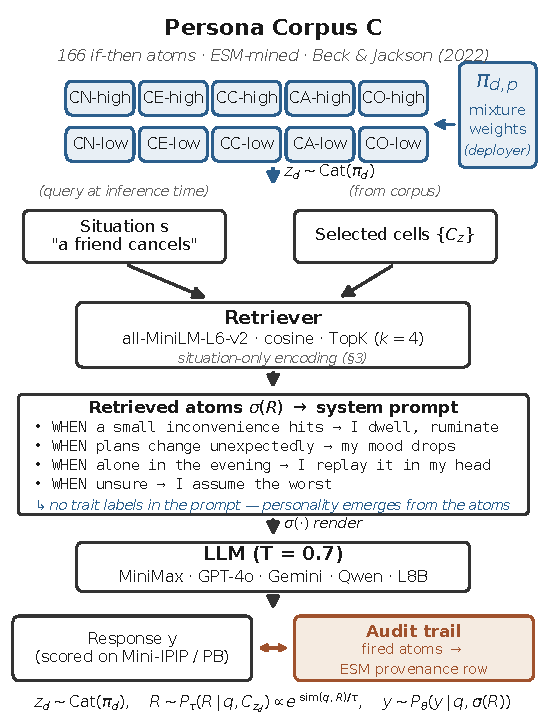
\includegraphics[width=\columnwidth]{figures/figure1_framework.pdf}
\caption{Persona-CAPS at inference. A persona is a corpus $C$ of \texttt{if-then} atoms organised into ten (dim, polarity) cells. Deployer-set mixture weights $\pi_{d,p}$ select active cells; the retriever encodes the query and each atom's situation field (\texttt{all-MiniLM-L6-v2}, cosine, top-$k{=}4$); retrieved atoms are rendered into a system prompt that contains \emph{no trait labels}; the LLM samples response $y$ at $T{=}0.7$; every fired atom is logged with provenance back to its ESM observation, yielding a per-response audit trail (\S~4.3). Conditional independencies, for a single dimension $d$ under control: $z_d \sim \mathrm{Cat}(\pi_d)$, $R \sim P_\tau(R \mid q, C_{z_d})$, $y \sim P_\theta(y \mid q, \sigma(R))$. The 5-D composition of \S~4.6 selects one $z_d$ per dimension and concatenates the five retrieved sets.}
\label{fig:framework}
\end{figure}
.
\begin{figure}[t]
\centering
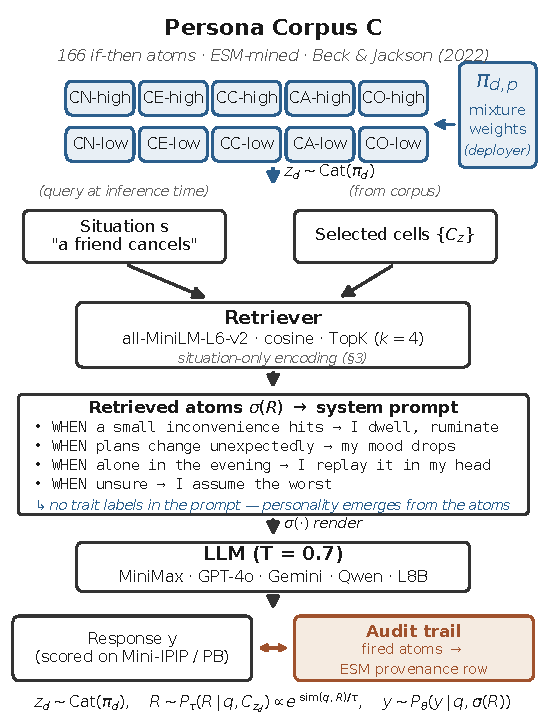
\includegraphics[width=\columnwidth]{figures/figure1_framework.pdf}
\caption{Persona-CAPS at inference. A persona is a corpus $C$ of \texttt{if-then} atoms organised into ten (dim, polarity) cells. Deployer-set mixture weights $\pi_{d,p}$ select active cells; the retriever encodes the query and each atom's situation field (\texttt{all-MiniLM-L6-v2}, cosine, top-$k{=}4$); retrieved atoms are rendered into a system prompt that contains \emph{no trait labels}; the LLM samples response $y$ at $T{=}0.7$; every fired atom is logged with provenance back to its ESM observation, yielding a per-response audit trail (\S~4.3). Conditional independencies, for a single dimension $d$ under control: $z_d \sim \mathrm{Cat}(\pi_d)$, $R \sim P_\tau(R \mid q, C_{z_d})$, $y \sim P_\theta(y \mid q, \sigma(R))$. The 5-D composition of \S~4.6 selects one $z_d$ per dimension and concatenates the five retrieved sets.}
\label{fig:framework}
\end{figure}


\textbf{Atoms, retrieval, agent.} A persona is a corpus $C = \{a_1, \ldots, a_n\}$ of \textit{if-then atoms}; each atom $a = (\text{situation},\allowbreak  \text{behavior},\allowbreak  [\text{affect}],\allowbreak  [\text{goal}],\allowbreak  [\text{dim}],\allowbreak  [\text{pol}])$ is two natural-language sentences plus optional metadata (in brackets), stored one per JSONL row --- \textit{the file is the persona}. Given a runtime situation $s$ we encode $s$ and each atom's \textit{situation field only} with \texttt{all-\allowbreak{}MiniLM-\allowbreak{}L6-\allowbreak{}v2} \cite{sbert2019} (384-dim, L2-normalised) and retrieve top-$k = 4$ atoms by cosine similarity; the agent renders these into a fixed system-prompt template (\S~\ref{app:A.1}) that contains \textbf{no trait labels}. Indexing the situation half forces a \textit{cross-target match} against the inventory item's behavioural description, foreclosing the tautological behavior-to-behavior lookup that would inflate \S~\ref{sec:4.1}. Fired atoms are logged alongside the response (\S~\ref{app:A.3}), and a localized corpus repair touches only the atoms the audit identifies --- no model retraining is involved.

\textbf{Baselines.} Two persona-as-string baselines: \textit{TraitPromptAgent} (single trait label) and \textit{PersonaDescriptionAgent} (~150-word character-card description, hand-authored without naming the trait). Two same-scaffolding ablations: \texttt{random\_\allowbreak{}demos} (chitchat atoms) and \texttt{wrong\_\allowbreak{}trait} (atoms from an orthogonal Big-Five dim at the same polarity). For \S~\ref{sec:4.4} we additionally use the \textit{Simple-Prompt} (SP) and \textit{$P^{\!2}$} paragraph-prompt baselines verbatim from \citet{NPTI}; \S~\ref{sec:4.5} adds a \textit{mixed-percentage prompt} baseline.

\textbf{Empirically grounded corpus from ESM data.} Atoms are mined from \citet{beck2022esm} (openESM \texttt{0060\_\allowbreak{}beck}, CC BY-NC 4.0) via a 6-step pipeline (\S~\ref{app:A.6}) that bins participants by trait quartiles, crosses eight DIAMONDS situation-perception items \cite{rauthmann2014diamonds} and 18 binary context flags against each behavioral item, retains $(\text{situation}, \text{behavior})$ cells with $|d_\text{high} - d_\text{low}| \geq 0.3$ (our operationalisation of \citet{mischel1995caps}'s if-then behavioral signature), and verbalises each into a first-person if-then atom via MiniMax-M2.7; every atom carries a \texttt{provenance} dict. \textbf{Released corpus}: 166 atoms across 10 (dim $\times$ polarity) cells, mean $|d| = 0.51$. \textbf{No-leakage validation} (\S~\ref{app:A.4}): trigram-Jaccard with any Mini-IPIP item $\leq 0.134$ ($0/20 \geq 0.20$); 16 / 20 items have their globally nearest atom in a \textit{non-target} cell.

\textbf{Locus of probability.} Equation (1) is an \textbf{operational mixture over prompting contexts}, not a likelihood of the black-box LLM: each summand is a concrete sampling pipeline (draw cell $z$, retrieve top-$k$, prepend, sample $y$ at $T=0.7$), with $\pi$ deployer-set. Softmax retrieval at $\tau = 1.0$ preserves $\approx$87\% of the deterministic top-$k$ spread (App.~\ref{app:C}). The four CAPS-theoretic design choices that distinguish this from generic RAG-prompting are operationalised in \S~\ref{sec:4.2} and \S~\ref{sec:4.3}.

\section{Experiments and Results}
\label{sec:4}

We address seven research questions targeting the \S~\ref{sec:1} contributions: trait fidelity (\S~\ref{sec:4.1}), content-specificity (\S~\ref{sec:4.2}), compositional editing (\S~\ref{sec:4.3}), PersonalityBench head-to-head (\S~\ref{sec:4.4}), continuous strength (\S~\ref{sec:4.5}), 5-D joint composition (\S~\ref{sec:4.6}), and audit-loop efficiency (\S~\ref{sec:4.7}). \S~\ref{sec:4.1}--\S~\ref{sec:4.6} establish standard-control parity; \S~\ref{sec:4.7} makes the governance argument. Diagnostic null and conditional-probability sweeps live in App.~\ref{app:B}--C.

\subsection{RQ1 --- Stable, measurable Big Five expression on Mini-IPIP, replicated across three vendors}
\label{sec:4.1}

\textbf{Mini-IPIP as a controlled diagnostic, not sufficient evidence.} Following the methodological cautions of \citet{serapio2023personality} and \citet{abdulhai2025consistent}, \S~\ref{sec:4.1} uses Mini-IPIP as a \textit{controlled diagnostic} of trait expression under a fixed prompt template across all conditions; we do \textit{not} treat its score as evidence that an LLM ``has'' the corresponding trait. The load-bearing behavioural evaluation is the \S~\ref{sec:4.4} head-to-head on free-response PersonalityBench against the same SP and $P^{\!2}$ baselines.

\textbf{Setup.} 20-item Mini-IPIP \cite{donnellan2006miniipip} (5-point Likert, theoretical spread range $\pm 4$) under five conditions (CAPS, \texttt{trait\_\allowbreak{}label}, \texttt{persona\_\allowbreak{}description}, \texttt{random\_\allowbreak{}demos}, \texttt{wrong\_\allowbreak{}trait}; \S~\ref{sec:3}) on three subject backends (MiniMax-M2.7-highspeed, hereafter MM; GPT-4o-2024-08-06; Gemini-2.5-Flash) at $T = 0.7$, $N = 5$ runs per cell. Bootstrap 95\% CIs (10,000 resamples) on per-run mean target spread $M(\text{high}) - M(\text{low})$; only \texttt{LLMClient} differs across backends.

\begin{table*}[t]
\centering
\fitwidth{\textwidth}{%
\begin{tabular}{lrrrrr}
\toprule
backend & \texttt{caps} & \texttt{trait\_\allowbreak{}label} & \texttt{persona\_\allowbreak{}desc} & \texttt{random\_\allowbreak{}demos} & \texttt{wrong\_\allowbreak{}trait} \\
\midrule
MiniMax-M2.7-highspeed & \textbf{+2.51} [+2.32, +2.73] & +2.69 [+2.62, +2.77] & +2.36 [+2.25, +2.51] & $-$0.01 [$-$0.06, +0.05] & $-$0.19 [$-$0.31, $-$0.07] \\
GPT-4o-2024-08-06 & \textbf{+3.74} [+3.69, +3.79] & +3.49 [+3.44, +3.55] & +3.53 [+3.50, +3.57] & $-$0.04 [$-$0.11, +0.03] & +0.08 [$-$0.03, +0.19] \\
Gemini-2.5-Flash & \textbf{+3.99} [+3.97, +4.00] & +3.77 [+3.71, +3.82] & +3.84 [+3.76, +3.92] & +0.06 [+0.01, +0.13] & $-$0.13 [$-$0.30, +0.02] \\
\bottomrule
\end{tabular}
}
\caption{Mini-IPIP target-dimension spread on three commercial backbones under CAPS retrieval vs. two prompt baselines and two scaffolding ablations. CAPS is the only condition that combines a competitive spread with a near-zero collapse on the \texttt{wrong\_trait} ablation. Bootstrap 95\% CIs from 10{,}000 resamples.}
\label{tab:rq1-ablation}
\end{table*}

\textbf{Observations.} CAPS \textit{beats} both string baselines with disjoint bootstrap CIs on GPT-4o and Gemini-Flash; on MiniMax CAPS ($+2.51$) and \texttt{trait\_\allowbreak{}label} ($+2.69$) have overlapping bootstrap CIs, so we do not resolve a difference between them at this sample size, and CAPS still beats \texttt{persona\_\allowbreak{}description} and both ablations. Cross-vendor Pearson $r$ on the full 25-cell per-(method, dim) spread grid is $\geq 0.92$ for every pair (full matrix in \S~\ref{app:A.7}), so the effect is a property of the representation, not of per-backend tuning.

\subsection{RQ2 --- Content-specificity ablations}
\label{sec:4.2}

RQ2 isolates whether the \S~\ref{sec:4.1} effect comes from CAPS's specific atom content or merely from having persona-shaped content in the system prompt. \textbf{Both ablations collapse to $\approx$ 0 on all three backends} (Tab.~\ref{tab:rq1-ablation}): \texttt{random\_\allowbreak{}demos} ranges $-0.04$ to $+0.06$ and \texttt{wrong\_\allowbreak{}trait} (the stronger control: same persona-like form, \textit{different trait content}) ranges $-0.19$ to $+0.08$, every CI excluding the smallest CAPS CI on the same backend by at least an order of magnitude --- ruling out both ``the effect is from in-context demonstrations'' and ``the effect is from any persona-shaped content occupying the system prompt.'' A cross-distribution check additionally rebuts the latent inventory-leakage worry: a \textit{circular-by-construction} IPIP-derived corpus (atoms paraphrased from IPIP-NEO-300 item phrasings, matched $N{=}3$) does not outperform Beck on Mini-IPIP (Beck $+2.33$ vs IPIP $+2.23$, MM) --- the abstract item bank does not yield stronger trait-spread than ESM-grounded situational atoms (full numbers in App.~\ref{app:B.3}).

\subsection{RQ3 --- Compositional editing: 10/10 directional moves from a worst-case opposing-pole base}
\label{sec:4.3}

\textbf{Setup.} For each (target dim, target polarity), we start from the corpus of the \textit{opposite} polarity (the hardest starting point), incrementally add 0 / 5 / 10 / 15 / 20 atoms from the target polarity, and re-administer the Mini-IPIP after each step ($N=3$ runs per step, mean reported, MiniMax-M2.7-highspeed). Beck v2 corpus throughout. All 10 conditions complete (raw payloads under \texttt{runs/\allowbreak{}rq3\_\allowbreak{}n3/\allowbreak{}}).

\textbf{10 / 10 conditions move the target in the predicted direction} (mean $|\Delta| = 1.38$ inventory points / 5); we additionally report a stricter $2\times$ off-target criterion (target $|\Delta| \geq 2\times$ max off-target $|\Delta|$) as an upper bound, which \textbf{4 / 10} conditions clear (high-N $5.08\times$, low-E $12.36\times$, low-A $6.00\times$, low-O $8.00\times$). The four strict winners are ``low''-targeted plus high $N$ --- edits travelling toward an off-default chat-model region; the six near-misses still move correctly but fight an off-target shift on RLHF-correlated traits (e.g., editing toward low-C drags neuroticism up by more than the target move itself). The same asymmetry recurs in \S~\ref{sec:4.4} and \S~\ref{sec:4.5}, triangulating the \textit{residual difficulty as a property of the chat model's prior, not of the representation}. Per-cell initial $\to$ final scores and per-cell off-target ratios in App.~\ref{app:A.8} (Table~\ref{tab:rq3-compositional}). Figure~\ref{fig:audit-case} shows this edit primitive on the \S~\ref{sec:1} corpus-build bug (fired-atom log localization, 2-row JSONL fix; Mini-IPIP $-0.50 \to +0.58$, $N=3$); \S~\ref{sec:4.7} makes the audit-and-fix loop systematic via controlled $K$-atom polarity injection.

% paper/latex/figures/figure2_case_study.tex
% §4.3 debug-and-fix audit case study. Drop into main_body via % paper/latex/figures/figure2_case_study.tex
% §4.3 debug-and-fix audit case study. Drop into main_body via \input{figures/figure2_case_study.tex}.
\begin{figure}[!t]
\centering
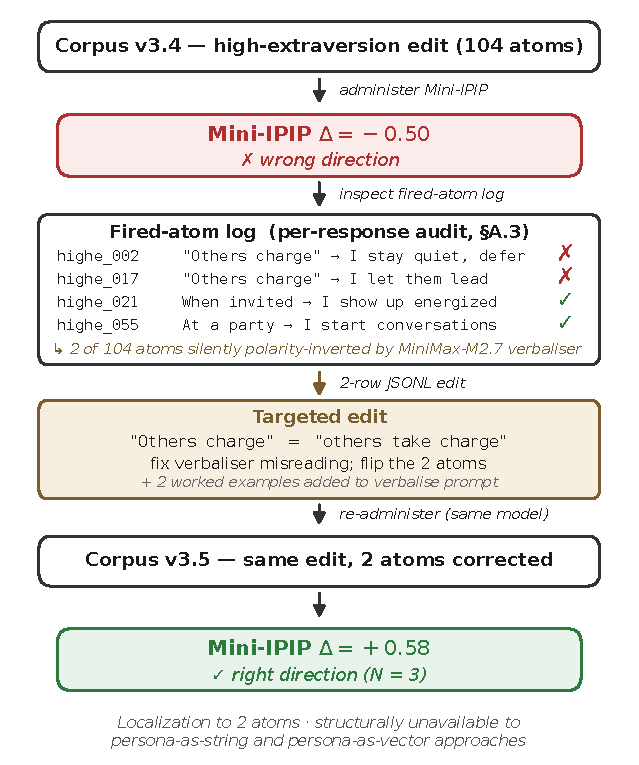
\includegraphics[width=\columnwidth]{figures/figure2_case_study.pdf}
\caption{The \S~4.3 debug-and-fix audit case at two-atom granularity. In an earlier corpus build (v3.4) the high-extraversion edit moved Mini-IPIP by \textbf{$-0.50$} (wrong direction); the fired-atom log localised the bug to \textbf{two atoms among the 104}, both reverse-keyed and both arising from the codebook phrase \texttt{"Others charge"}, which MiniMax-M2.7 misread as \texttt{"others are charging at me"} rather than \texttt{"others take charge"}, silently inverting the polarity of their first-person verbalisation. A two-row JSONL edit fixed the verbalisations; the same edit on the same model now produces \textbf{$+0.58$} ($N{=}3$). Localisation to two atoms is structurally available to a contingency-level retrieval representation and unavailable to persona-as-string and persona-as-vector approaches.}
\label{fig:audit-case}
\end{figure}
.
\begin{figure}[!t]
\centering
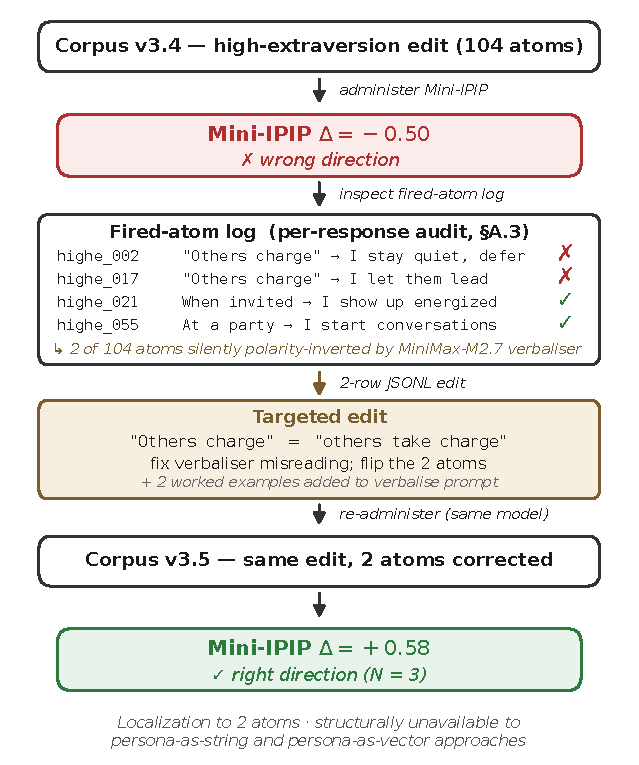
\includegraphics[width=\columnwidth]{figures/figure2_case_study.pdf}
\caption{The \S~4.3 debug-and-fix audit case at two-atom granularity. In an earlier corpus build (v3.4) the high-extraversion edit moved Mini-IPIP by \textbf{$-0.50$} (wrong direction); the fired-atom log localised the bug to \textbf{two atoms among the 104}, both reverse-keyed and both arising from the codebook phrase \texttt{"Others charge"}, which MiniMax-M2.7 misread as \texttt{"others are charging at me"} rather than \texttt{"others take charge"}, silently inverting the polarity of their first-person verbalisation. A two-row JSONL edit fixed the verbalisations; the same edit on the same model now produces \textbf{$+0.58$} ($N{=}3$). Localisation to two atoms is structurally available to a contingency-level retrieval representation and unavailable to persona-as-string and persona-as-vector approaches.}
\label{fig:audit-case}
\end{figure}


\subsection{RQ4 --- Head-to-head on the NPTI PersonalityBench protocol (3 backbones $\times$ 3 methods, uniform GPT-4o judge)}
\label{sec:4.4}

\textbf{Setup.} We replicate NPTI's PersonalityBench evaluation \cite{NPTI} (459 scenario questions, 1--5 LLM-as-judge rating, per-cell pool 89--100) and extend it to a \textbf{3$\times$3 head-to-head}: \textbf{subjects} MM, Gemini-2.5-Flash, \textbf{Llama-3-8B Q4\_K\_M} (NPTI's primary backbone, via Ollama); \textbf{methods} CAPS, \textit{Simple-Prompt} (SP) and \textit{$P^{\!2}$} \cite{jiang2023p2} paragraph-prompt (one description per call from \citet{NPTI}'s 800-description bank, 80 per cell); \textbf{judge} GPT-4o-2024-08-06 ($T=0$), held constant across all 9 cells; \textbf{budget} 50 q per (trait $\times$ polarity) cell, 4,500 judged responses total (App.~\ref{app:A.9} aggregation; raw payloads \texttt{runs/\allowbreak{}personalitybench\_\allowbreak{}*\_\allowbreak{}scored/\allowbreak{}}).

\textbf{Headline 3$\times$3 (apples-to-apples: same judge, same $N$, same templates).} All nine cells sit high on the 10-point scale and span less than a point within any backbone, so the head-to-head turns on \textit{which} traits each method moves and \textit{whether} that pattern survives a change of backbone, not on aggregate magnitude. Per-backbone, per-trait scores are in Tables~\ref{tab:pb-mm}--\ref{tab:pb-l8b} (App.~\ref{app:A.9}).

\textbf{Two findings.} \textbf{(i) CAPS exceeds SP on every backbone} ($+0.86, +0.71, +0.50$; mean $+0.69/10$), with the lift concentrated on Conscientiousness and Openness ($+0.96$ and $+1.85$ mean across the three backbones) --- the same two traits IRiS / NPTI document SP under-expressing. The CAPS$-$SP gap is therefore a generic property of substituting situated atoms for label-only prompting, not a single-backbone artefact. \textbf{(ii) The CAPS$-$$P^{\!2}$ gap is within $0.11$ pt on the two commercial backbones and closes monotonically as backbones strengthen} (L8B $-0.37$ $\to$ Gem $0.00$ $\to$ MM $+0.11$). A \texttt{-\allowbreak{}-\allowbreak{}strip-\allowbreak{}affect-\allowbreak{}metadata} template ablation on L8B recovers about a third of the residual, and the recovery is concentrated on the N/O cells \S~\ref{app:A.4.1} identifies as driving the residual, with a trade-off on $E$ rather than a unilateral gain. That cell-level agreement, rather than the size of the score change, is what identifies atom \textit{rendering} and not retrieval as the mechanism; the ablation is a diagnostic, not a deployment recommendation.

\textbf{Validation.} \citet{NPTI} publish SP $8.39$ and $P^{\!2}$ $9.43$ for this protocol, as tabulated by \citet{IRiS}; our SP-on-L8B ($8.66$) and $P^{\!2}$-on-L8B ($9.53$) sit $+0.27$ and $+0.10$ above them, a drift consistent with our 50-q-per-cell cap and Q4 quantisation (Limitations). CAPS at $9.16$ ($9.28$ with the \S~\ref{app:A.4.1} strip ablation) clears published SP but stays below the model-internals methods on the same protocol (NPTI $9.43$, IRiS $9.59$), which need weight-level access. The \textit{relative} CAPS$-$$P^{\!2}$ gap on the held-constant judge is the load-bearing comparison.

\phantomsection\label{sec:4.4.1}
\textbf{\S~4.4.1 Robustness.} Three confounds could each manufacture the CAPS$-$SP lift on their own: a judge drawn from $P^{\!2}$'s model family, CAPS's shorter answers, and an induction source shared between $P^{\!2}$ and the benchmark. App.~\ref{app:A.10} bounds all three, and none is large enough to do so --- swapping in a same-vendor judge moves the CAPS lift by under a tenth of a point, the strongest verbosity correlations sit in the baselines and not in CAPS, and $P^{\!2}$ sits closer to the benchmark's IPIP-NEO source in semantic space than the independently mined atom corpus does, with no surface-text overlap in either direction. The latter two residuals run \textit{against} CAPS, and a two-rater human pack (App.~\hyperref[app:A.10.1]{A.10.1}) agrees on the sign of the gap.

\subsection{RQ5 --- Continuous personality strength control via mixture weights $\pi_d$}
\label{sec:4.5}

Beyond polarity, do the mixture weights $\pi_{d,p}$ act as a continuous knob for the \textit{expected} trait \textit{strength}? (The within-cell $\tau_r$ moves spread only $-12.7\%$ across its range --- App.~\ref{app:C} Sweep A.)

\textbf{Setup.} Per dim $d$, activate \texttt{high\_\allowbreak{}d} / \texttt{low\_\allowbreak{}d} with weights $(w, 1-w)$, $w \in \{0, 0.25, 0.5, 0.75, 1\}$; \texttt{JointCapsAgent} draws one cell per query, \texttt{top\_\allowbreak{}k\_\allowbreak{}per\_\allowbreak{}dim = 4}. Three commercial backends (Gem, GPT-4o, MM) at $T = 0.7$, $N = 3$ runs per $w$ --- 225 administrations. We use $k = 4$ throughout as a representative control--auditability working point rather than a tuned optimum: an endpoint sweep over $k \in \{2, 4, 8\}$ (App.~\hyperref[app:A.9.9]{A.9.9}) leaves the achievable range nearly flat across a fourfold change in budget, so a larger $k$ buys almost no additional control while adding a row to every audit trail.

\textbf{Result --- monotonic control on every dimension on every vendor.} All 15 (vendor $\times$ dim) cells are \textbf{strictly monotonic in $w$} with per-cell Spearman $\rho = +1.000$, traversing $\geq 2.25$ inventory points end-to-end (joint random-ordering null $\approx 6.5 \times 10^{-32}$). Across vendors the \textit{shape} of the curve transfers almost exactly while its \textit{height} does not: every pairwise cross-vendor correlation among the three stays above $+0.97$ --- and above $+0.85$ across all five backbones once the open-weight replications are folded in (App.~\ref{app:A.7}) --- yet the mean spreads differ by more than a full inventory point between the widest and narrowest backbone. What transfers is the ordering of $\pi_d$ settings, not a fixed trait level per setting; the absolute range a backbone can reach is a property of its instruction-tuned prior. Full grids in App.~\hyperref[app:A.9.5]{A.9.5} (Table~\ref{tab:pi-grid-commercial}); open-weight replications in App.~\hyperref[app:A.9.6]{A.9.6}--7.

\textbf{What $\pi_d$ controls.} For the dimension being swept, each query samples \textit{one} polarity cell according to $\pi_d$, so the monotonicity above is the \textbf{expected trait level over repeated generations}, not interpolation within a single response. This aggregate reading is the one CAPS asks for: the theory locates personality in contingencies stable \textit{across occasions}, not in a fixed intensity realised within every act. An exploratory three-arm pilot asks whether $\pi_d$ could instead be realised \textit{within} a single prompt: retrieving both polarity cells into one prompt does narrow the response distribution (extreme-rating share $64\% \to 28\%$, and to $11\%$ once a target-free integration instruction is added), but the mean curves lose strict monotonicity and that instruction also compresses the endpoints, so the deployed knob remains the frequency axis (App.~\hyperref[app:A.9.10]{A.9.10}).

\textbf{A mixed-percentage prompt reaches the same 1-D control surface.} Asking a model directly for \textit{``X\% high pole and (100$-$X)\% low pole''} is monotonic on 14 of 15 cells and, cell by cell (Table~\ref{tab:caps-vs-promptbase}, App.~\hyperref[app:A.9.11]{A.9.11}), matches CAPS on end-to-end range and on off-target leakage while being marginally the better calibrated of the two. On the strength axis taken by itself, CAPS is therefore not the wider or the cleaner knob. What the percentage prompt cannot do is report which retrieved unit produced a given response, or let a deployer edit that unit and re-verify --- the properties \S~\ref{sec:4.7} measures. The control surface itself replicates on open-weight backbones and on a distilled reasoning subject (Qwen3.5-9B, Llama-3-8B, DeepSeek-R1-Distill-Qwen-14B; App.~\hyperref[app:A.9.6]{A.9.6}--8).

\subsection{RQ6 --- Joint 5-D Big-Five composition: $\pi$ as a multi-trait control surface}
\label{sec:4.6}

\textbf{Setup.} \texttt{JointCapsAgent} retrieves $k_\text{per dim}$ atoms from each of the five cells the profile requests (one endpoint polarity per dimension, $\pi_d \in \{0,1\}$), concatenated into one prompt. We evaluate \textbf{7 Big-Five profiles} --- HHHHH, its 5 single-flips (one trait reversed against an otherwise prosocial prior), and LLLLL (anti-prior stress) --- at $N{=}3$ runs and $k{\in}\{3, 4\}$, against a 5-D $P^{\!2}$ baseline stacked from \citet{NPTI} single-trait paragraphs (construction in App.~\ref{app:C.4}).

\textbf{How to read the table.} Direction-match asks only whether each of the five dimensions moved the way it was asked to --- the criterion a deployer can check without a calibrated scale. It is deliberately coarse: a dimension counts as matched once it clears the scale midpoint by $0.25$ inventory points in the prescribed polarity, however far short of the pole it stops. The finer measures in App.~\ref{app:C.4} (intensity, per-flip specificity, swing, cross-dimension drift) do not reverse the head-to-head, though $P^{\!2}$ does hold a small intensity-axis lead on both backbones, which we attribute to its explicit Big-Five vocabulary matching the Mini-IPIP item language rather than to better composition.

\begin{table*}[t]
\centering
\fitwidth{\textwidth}{%
\begin{tabular}{lrr}
\toprule
method & MM (all 7 / excl.\ LLLLL / LLLLL) & Gem (all 7 / excl.\ LLLLL / LLLLL) \\
\midrule
CAPS ($k_\text{per dim}{=}4$) & \textbf{0.91} / \textbf{0.93} / 0.73 & \textbf{0.97} / \textbf{1.00} / 0.80 \\
$P^{\!2}$ (NPTI stacked, App. \ref{app:C.4}) & 0.95 / 0.96 / \textbf{0.93} & 0.99 / 0.99 / \textbf{1.00} \\
\bottomrule
\end{tabular}
}
\caption{Joint 5-D Big-Five composition head-to-head on two commercial backbones (MM, Gem) at $k_\text{per dim}{=}4$. Direction-match rate over 7 profiles $\times$ $N{=}3$ runs; \texttt{excl. LLLLL} removes the anti-prior all-low profile; \texttt{LLLLL} is the anti-prior cell only. Full grid (k=3 and k=4, per-profile, intensity, specificity) in Table~\ref{tab:p2-joint-5d-headtohead} (App. \ref{app:C.4}).}
\label{tab:rq6-joint-headtohead}
\end{table*}

\textbf{On the 12 non-all-low profile--backbone cells the methods reach the same direction-match} (HHHHH + 5 single-flips $\times$ 2 backbones): 2 CAPS wins, 7 ties, 3 $P^{\!2}$ wins; overall $+1$ pp on Gemini and $-3$ pp on MM. The remaining 2 cells are LLLLL --- adversarial against the chat model's RLHF prior on every dim --- where explicit label-override prompts are structurally suited: a complementary regime, not a unified loss ($-20$ pp on both backbones; Tab.~\ref{tab:rq6-joint-headtohead}).

\subsection{RQ7 --- Audit-loop efficiency: bug injection, localization, and atom-level repair}
\label{sec:4.7}

\textbf{Motivation and experimental question.} \S~\ref{sec:4.1}--4.6 measure \textit{what} each persona method produces; \S~\ref{sec:4.7} measures \textbf{the governance interface}: what happens when the persona representation contains a contradiction, and what each method can do about it. We inject $K$ polarity-inverted atoms into the persona corpus and ask, of each representation: can it detect the corruption (sanity gate), localize the bad atoms, and repair them without collateral damage to other traits? Two CAPS audit workflows and three $P^{\!2}$ baselines are compared on localization precision / recall, post-fix restoration of the clean Mini-IPIP profile, edit footprint, and off-target preservation. Subject backbone MiniMax-M2.7-highspeed ($T = 0.7$), 3 seeds per (cell, $K$); driver and aggregation scripts in \texttt{scripts/\allowbreak{}audit\_\allowbreak{}loop/\allowbreak{}} (\texttt{aggregate.py}); raw payloads under \texttt{runs/\allowbreak{}audit\_\allowbreak{}loop/\allowbreak{}}. Mini-IPIP shifts here are a representation-shift proxy (per-cell reproducible), not a trait measurement (cf. \S~\ref{sec:4.1}).

\textbf{Pollution protocol (targeted strategy).} \textbf{For retrieval-based audit we deliberately construct the worst case:} for each (dim, polarity) cell we draw $K \in \{5, 10, 15\}$ atoms from the target cell and rewrite each \texttt{behavior} field via GPT-4o ($T=0$, strict-JSON, $\geq 1$ retry, hard-reject pure-negation rewrites) into the opposite polarity --- situation, affect, and visible metadata (\texttt{polarity}, \texttt{target\_\allowbreak{}dimension}) preserved verbatim, so the metadata still claims the atom is on-polarity. A condition is sanity-passing iff the polluted-vs-clean Mini-IPIP shift on the target dim has $|\Delta\bar{s}| \geq 1.0$ point \textit{and} at least two of the four target-dim items cross the scale midpoint (\textit{direction-match rate} $\leq 0.7$).

\textbf{Trait-asymmetric editability --- and its diagnostic value.} Mean $|\Delta\bar{s}|$ across the 9 (K, seed) conditions per cell: high-E $2.53$, low-O $2.89$, high-N $0.92$, low-A $0.83$, low-C $0.47$ (Tab.~\ref{tab:rq7-mm-sanity}). MiniMax's conscientiousness prior dominates even when 15 / 31 atoms are inverted, so the audit-loop runs on the four cells that \textit{can} be polluted (E, A, N, O). This asymmetry is itself a finding: corpus-pollution sensitivity doubles as a probe for RLHF-locked dimensions --- that low-C resists $K=15$ injection tells a deployer MM has \textit{overdetermined} conscientiousness. C-cell scope in Limitations.

\textbf{Five audit workflows, identical subject + query stream.} \textbf{CAPS-A} (incident-driven, per-response): for each Mini-IPIP item where polluted disagrees with clean in direction, flag the atom in the agent's fired-atom log whose situation most closely matches the item --- sparse by construction. \textbf{CAPS-B} (scheduled, corpus-metadata sweep): GPT-4o re-classifies every atom's behavior into $(\text{dim}, \text{polarity})$ and flags any atom whose classification disagrees with its stored \texttt{polarity} --- one-shot batch over the corpus. \textbf{$P^{\!2}$-Oracle} (upper bound): the auditor is handed the $K$ ground-truth flipped sentences in the matching $P^{\!2}$ paragraph and edits exactly those. \textbf{$P^{\!2}$-Blind}: entire D-paragraph regenerated from the trait-target prompt; no per-atom editable unit. \textbf{$P^{\!2}$-Detect}: same inventory-disagreement signal as CAPS-A, plus GPT-4o is asked which sentences are most likely responsible --- the closest $P^{\!2}$ counterpart to CAPS-A.

\textbf{$P^{\!2}$ leaves sanity-gate failures on 2 of 4 cells --- a representation-level finding. Over individual $(K, \text{seed})$ conditions $P^{\!2}$-sanity passes $0/9$ on MiniMax low-openness across $K \in \{5, 10, 15\}$ and $1/3$ on high-neuroticism at $K = 15$; only low-openness has no passing condition at all.} When the same $K$ inverted behaviors are stitched into the surrounding $\sim 320$-word $P^{\!2}$ paragraph, the unchanged trait declaration dilutes them and the resulting persona is indistinguishable from clean $P^{\!2}$ on the target dim ($|\Delta\bar{s}| < 1.0$): \textbf{retrieval surfaces corpus pollution that paragraph dilution masks}. $P^{\!2}$ metrics below are therefore reported on the matching sanity-pass subset; CAPS metrics use the full sanity-passing CAPS set.

\begin{table*}[t]
\centering
\fitwidth{\textwidth}{%
\begin{tabular}{llllll}
\toprule
cell (n) & CAPS-A P / R, fix, edits & CAPS-B P / R, fix, edits & $P^{\!2}$-Oracle P / R, fix, edits & $P^{\!2}$-Blind fix, edits & $P^{\!2}$-Detect P / R, fix, edits \\
\midrule
high-E (6) & \textbf{1.00 / 0.33}, \textbf{5 / 6}, \textbf{4} & 0.92 / 1.00, 6 / 6, 12.5 & 1.00 / 1.00, 6 / 6, 12.5 & 6 / 6, full $\sim 320$ w & 1.00 / 1.00, 4 / 6, 12.5 \\
high-N (3) & 1.00 / 0.40, 1 / 3, 6 & 1.00 / 1.00, 2 / 3, 15 & 1.00 / 1.00, 1 / 1, 15 & 1 / 1, full & 1.00 / 1.00, 1 / 1, 15 \\
low-A (2) & 0.42 / 0.15, 0 / 2, 2 & 0.92 / 1.00, \textbf{1 / 2}, 12.5 & 1.00 / 1.00, 0 / 2, 12.5 & 0 / 2, full & 1.00 / 1.00, 0 / 2, 12.5 \\
low-O (9) & 0.80 / 0.44, \textbf{6 / 9}, 4 & 0.68 / 1.00, 4 / 9, 10 & --- & --- & --- \\
\bottomrule
\end{tabular}
}
\caption{Localization, fix success, edit footprint, and off-target preservation over the four CAPS-sanity-passing cells. Means over seeds and $K$; n per cell. $P^{\!2}$-sanity pass rates: high-E 6/6, low-A 2/2, high-N 1/3, low-O 0/9 (\S~\ref{sec:4.7}); em-dash = workflow unavailable (low-O $P^{\!2}$-sanity fails). Low-A: 2 of the 9 MM (K, seed) conditions pass the sanity gate (K=10 and K=15, both seed 3; Limitations); reported on those 2. Bold = CAPS-A's sparse-edit signature: 4-atom edits, $0.32\times$ the $P^{\!2}$-Oracle footprint at comparable fix-success on high-E.}
\label{tab:rq7-audit}
\end{table*}

\textbf{Three localization patterns.} (i) \textbf{Locator B achieves $R = 1.00$ across all four cells}, with precision cell-dependent ($0.68$--$1.00$). On low-openness $P$ rises monotonically with $K$ ($0.45$ / $0.71$ / $0.88$ at $K = 5$ / $10$ / $15$), consistent with a roughly fixed false-positive count diluted by rising true positives. (ii) \textbf{Locator A is a sparse high-precision triage tool on extraversion and neuroticism} ($P = 1.00$, $R = 0.33$--$0.40$, 4--6 atoms flagged out of $K = 10$--$15$) but \textbf{degrades on low-agreeableness} ($P = 0.42$, $R = 0.15$; downstream CAPS-A fix $0/2$ on this cell): IPIP-A items semantically overlap multiple Big-Five dimensions and the fired-atom signal becomes diffuse. Locator A is cell-dependent --- on low-openness it reaches $P = 0.80$. (iii) \textbf{$P^{\!2}$-Oracle / $P^{\!2}$-Detect score $P{=}R{=}1.00$ on the three cells that have at least one $P^{\!2}$-sanity-passing condition}, but only because Oracle gets ground truth and Detect labels sentences on a 26\nobreakdash--39-atom corpus with the cell label visible --- structurally easier than CAPS's locator task.

\textbf{Two repair patterns the localization table hides.} (i) \textbf{On low-agreeableness, CAPS-B (fix 1 / 2) is the only workflow that recovers the clean persona}; $P^{\!2}$-Oracle, $P^{\!2}$-Blind, and $P^{\!2}$-Detect each achieve $0 / 2$ fixes despite Oracle being handed ground-truth atom IDs. The bottleneck is not localization: $P^{\!2}$ paragraph rewrites cannot carry the ESM-style first-person contingency the CAPS persona uses, even when the editor knows exactly what to change. (ii) \textbf{On low-openness CAPS-A (6 / 9) outperforms CAPS-B (4 / 9)} despite Locator B's perfect recall --- fix quality is bottlenecked by off-target spillover from editing 10--15 atoms at once, not by missing the ground-truth set.

\textbf{Off-target preservation: CAPS-A best, $P^{\!2}$-Detect and $P^{\!2}$-Blind worst} (mean $|\Delta\bar{s}|$ on four non-target dims). On the three cells where every workflow ran (high-E, high-N, low-A): CAPS-A $0.31$, CAPS-B $0.36$, $P^{\!2}$-Oracle $0.34$, $P^{\!2}$-Detect $0.44$, $P^{\!2}$-Blind $0.43$ (Tab.~\ref{tab:rq7-mm-offtarget}); $P^{\!2}$-Blind drifts $\sim 40\%$ more than CAPS --- the quantitative cost of paragraph-as-smallest-editable-unit. Including low-O CAPS-A grand mean $0.32$.

\textbf{Cross-vendor subject replication.} Across $13/13$ paired sanity-passing seeds the GPT-4o subject's CAPS-A flag set restores atoms with byte-identical per-seed character counts to the MiniMax subject (Tab.~\ref{tab:rq7-xvendor-byteid}) --- the edit unit is a property of the representation, not the subject. Full GPT-4o grid (off-target, $P^{\!2}$-Detect structural footprint, $P^{\!2}$-sanity regime-dependence): App.~\ref{app:A.11}~(i)--(iv).

\textbf{What the repair loop does and does not guarantee.} The workflow is \textit{localize--intervene--verify} at atom granularity: the audit marks candidate atoms, the intervention edits the \texttt{behavior} field of exactly those, and re-administering Mini-IPIP checks whether the clean profile is restored. Crucially, \textbf{there is no optimality guarantee before that verification step} --- a flagged edit is a hypothesis, and the fix-success columns above are the rate at which it survives checking. We claim an atom-granular localize--intervene--verify workflow, not root-cause analysis and not automated repair. Generating candidate fixes with verification in the loop --- propose, re-administer, revise until the profile is restored --- is the natural next step.

\textbf{Summary.} Three conclusions follow; exact per-cell values in Tab.~\ref{tab:rq7-audit}, Tab.~\ref{tab:rq7-xvendor-byteid} and App.~\ref{app:A.11}. First, \textbf{the representation decides whether corruption is visible at all}: a polluted paragraph still reads as Mini-IPIP-clean, while the same corruption is detectable once the persona is retrieved atom by atom. Second, \textbf{it decides how much must be rewritten to repair it}: CAPS-A restores the clean profile by editing a handful of flagged atoms where the paragraph baselines regenerate a whole one, with the least off-target drift of any workflow tested --- a contrast that survives a change of subject backbone, where CAPS-A's flag sets reproduce byte-for-byte. Third, \textbf{the choice of audit mode is operational, not a quality ranking}: Locator B's exhaustive recall fits scheduled sweeps, Locator A's sparse precision fits incident-driven triage, and neither dominates. Scope limits in Limitations.

\section{Discussion}
\label{sec:5}

Persona-CAPS reframes the persona representation from a control knob into an inspectable, editable, repairable artefact. \S~\ref{sec:4.5}--4.6 show that retrieval reaches the strongest paragraph baselines everywhere except the all-low stress profile; \S~\ref{sec:4.7} shows the same retrieval surfaces, locates, and repairs corpus-level pollution at $\sim 1/3$ paragraph-baseline footprint. The combination --- controllable and auditable through the same representation --- is what the title claims and what neither persona-as-string nor persona-as-vector currently delivers in a single deployable interface; $P^{\!2}$ has a clear edge on the weaker L8B backbone (\S~\ref{sec:4.4}) and on the adversarial all-low (LLLLL) profile; over the non-all-low profiles the backbone-level direction-match aggregates differ by at most 3 pp (\S~\ref{sec:4.6}).

\textbf{Paragraph representations can mask corpus corruption, and offer no sub-paragraph repair unit.} $K{=}15$ atoms inverted in a $\sim 320$-word $P^{\!2}$ paragraph leave the persona Mini-IPIP-clean --- corruption invisible at the representation level (\S~\ref{sec:4.7} $P^{\!2}$-sanity passes $0/9$ on MM low-O); retrieval surfaces it.

\textbf{Beyond persona control.} Nothing in the localize--intervene--verify loop is specific to personality: it requires only that the conditioning signal be assembled from \textit{human-readable retrieval units}. We therefore expect it to extend to other controlled-generation tasks built that way, such as style and register specifications or safety policies decomposed into retrievable rules. Persona control is the only setting we evaluate here.



% ACL/ARR formatting: Limitations + Ethical Considerations live BETWEEN
% Conclusion and References as unnumbered \section* (per ACLPUB guide,
% https://acl-org.github.io/ACLPUB/formatting.html). They do NOT count
% against the 8-page main-body budget.
\phantomsection\label{sec:limitations}
\section*{Limitations}

\begin{itemize}
\item \textbf{Reproduction drift and judge saturation.} \S~\ref{sec:4.4} holds the GPT-4o-2024-08-06 judge constant across all 9 cells so relative gaps are reliable, but \textit{absolute} /10 numbers drift slightly between papers (our SP- and $P^{\!2}$-on-L8B are $+0.27$ and $+0.10$ above the values published for this protocol by \citet{NPTI}, plausibly from our 50-q-per-cell sampling cap and Q4 quantisation); $P^{\!2}$ and CAPS both saturate the judge above the 9.0 tier on $A_\text{high}$ / $E_\text{high}$. The \S~\ref{sec:4.4} cross-judge check ($r = +0.951$; judge-swap sensitivity $0.08/10$, App.~\hyperref[app:A.10.1]{A.10.1}) and the preliminary human-validation packs bound these together.
\item \textbf{Adversarial-prior LLLLL profile.} On the all-low 5-D profile (against the chat model's RLHF prior on every dimension simultaneously) the stacked-paragraph $P^{\!2}$ baseline holds a $20$ pp edge over CAPS-$k{=}4$ on both commercial backbones, the regime where explicit \textit{``hostile, careless, closed-minded''} label-override prompts are structurally suited; the backbone-level aggregates over the 12 non-all-low cells differ by at most 3 pp (\S~\ref{sec:4.6}). Two remedies are available for this regime, and we would prioritise them in this order. First, an \textbf{adaptive anti-prior atom budget}: raise $k_\text{per dim}$ on exactly those dimensions where the requested polarity opposes the backbone prior, spending retrieval capacity where the prior resists and leaving the label-free interface --- the property the governance argument rests on --- intact. Only as a fallback would we prepend an explicit high-level directive to the retrieved atoms, which recovers paragraph-baseline behaviour on LLLLL at the cost of reintroducing the trait label that CAPS is designed to avoid. The absolute range and trait-specific shape of $\pi_d$ curves remain vendor-specific, so a deployer reads $w$ off a per-vendor calibration curve.
\item \textbf{Response-length asymmetry vs NPTI-verbatim baselines.} CAPS responses are systematically shorter than SP / $P^{\!2}$, a consequence of the \S~\ref{app:A.1} ``concise unless invited to elaborate'' design (so responses stay auditable against the small set of fired atoms) compounded on L8B Q4 by an atom-regurgitation early-termination failure (\S~\ref{app:A.4.1}). The two length-controlled re-analyses summarised in \S~\ref{sec:4.4} and detailed in App.~\ref{app:A.10} (per-item partial correlation and length-matched bootstrap) leave the \S~\ref{sec:4.4} conclusion intact, but the verbosity gap remains a confound and the human-eval pack is small. A future \texttt{-\allowbreak{}-\allowbreak{}match-\allowbreak{}length} CAPS variant generating verbosity-matched responses at decode time would close the asymmetry without the post-hoc bootstrap and is the natural follow-up.
\item \textbf{Atom-budget coupling in joint-persona mode.} With \texttt{top\_\allowbreak{}k\_\allowbreak{}per\_\allowbreak{}dim = 1}, single-trait personas on traits where the LLM has a strong opposing prior (most clearly high neuroticism on instruction-tuned chat models) degrade to a 33\% direction-match rate (App. \ref{app:C} Sweep C); the \S~\ref{sec:4.1} / \S~\ref{sec:4.3} single-cell experiments use $k = 4$ and show no such effect. Recommended joint-deployment lower bound is $k_\text{per dim} \geq 2$.
\item \textbf{Semantic conflict among co-retrieved atoms.} Retrieval scores atoms independently against the situation, so nothing in the current pipeline prevents one query from surfacing two atoms whose \texttt{behavior} fields pull in incompatible directions --- most likely in joint 5-D mode, where cells from several dimensions are drawn concurrently. Conflict with the \textit{backbone prior} we do measure, and it dampens rather than reverses (\S~\ref{sec:4.6}); conflict \textit{among the retrieved atoms themselves} is a distinct failure mode we do not quantify here. The mitigation the architecture already affords is a pre-generation pairwise contradiction check over the retrieved set, followed by compatibility-aware reranking --- or abstention, when no mutually consistent subset exists. Consistent with the governance interface, that decision would itself be written to the audit log, so a deployer can see which atoms were suppressed and why rather than inferring it from the response.
\item \textbf{Construction bottleneck, encoder, and missing backbones.} The corpus has to come from somewhere --- we use ESM-derived atoms for reproducibility; the companion repo includes scaffolding for human-authored and dialogue-extracted corpora we did not evaluate. The empirical \textit{selection} of atoms is data-driven (Cohen's $d \geq 0.3$ cells from openESM \texttt{0060\_\allowbreak{}beck}), but the \textit{linguistic realisation} is model-generated (MiniMax-M2.7); the \S~\ref{sec:4.3} audit case study shows this verbalisation step can silently invert polarity (and that the fired-atom log makes such errors locatable and one-row-fixable). A controlled comparison of template-rendered, human-authored, and LLM-verbalised atoms over the same selection set is future work. The retrieval encoder (\texttt{all-\allowbreak{}MiniLM-\allowbreak{}L6-\allowbreak{}v2}) is small and fast; a stronger encoder fine-tuned on situation paraphrasing would likely tighten App. \ref{app:B}'s $W$ statistic. Anthropic Claude is not included in this submission; the sweep covers three commercial backbones (MiniMax, GPT-4o, Gemini) and three open-weight ones (Llama-3-8B, Qwen3.5-9B, DeepSeek-R1-Distill-Qwen-14B). Our atoms use a two-component reduction $(\text{situation}, \text{behavior})$ of Mischel's full CAU (encodings, expectancies, beliefs, goals, plans); the framework supports the extension.
\item \textbf{Corpus demographic scope.} The if-then atoms are mined from \texttt{0060\_\allowbreak{}beck} (Beck \& Jackson 2022), an undergraduate ESM sample at a single US university (full participant demographics in the source paper). The Big-Five trait \textit{labels} used to select atoms generalize cross-culturally in the personality-psychology literature, but the \textit{situational triggers} and \textit{behavioral expressions} in the mined atoms reflect this population's daily contingencies and are unlikely to transfer verbatim to non-US, non-undergraduate, or non-anglophone deployment contexts. Re-mining from population-appropriate ESM data is supported by the open pipeline (selection + verbalisation, App.~\ref{app:A.6}) at the same cost profile as the Beck reproduction; corpus drift between source population and deployment population is a deployment-time configuration concern, not a code change.
\item \textbf{Audit-loop scope and corpus-size constraints.} The main \S~\ref{sec:4.7} table is run on a single subject (MiniMax-M2.7-highspeed); a GPT-4o-2024-08-06 cross-vendor subject grid reproduces the edit-footprint and off-target contrasts on every cell and establishes byte-identical CAPS-A flag sets across the paired sanity-passing seeds (App.~\ref{app:A.11}). A second cross-vendor subject family (e.g.\ Claude) and the lower-$K$ extension on the other three cells are not in this submission. The \S~\ref{sec:4.7} $P^{\!2}$-sanity-on-low-O finding does not replicate on GPT-4o, so $P^{\!2}$'s failure mode is subject-dependent: paragraph dilution masks corpus pollution on the more conservative subject, while on the more compliant one the rewritten paragraph does move the persona behaviorally yet still offers no persistent, provenance-linked sentence-level edit unit, at the cost of over a full Likert point of off-target drift. The \S~\ref{sec:4.7} claim is therefore the disjunction of the two regimes rather than the MM-specific version; per-condition figures are in App.~\ref{app:A.11}~(iv). Two cells constrain scope: low-conscientiousness cannot be polluted at our budget, so the sanity-passing set is E, A, N, O (\S~\ref{sec:4.7}), and low-A contributes only two sanity-passing seeds, one at $K{=}10$ and one at $K{=}15$, reported with explicit small-$n$ caveats (Tab.~\ref{tab:rq7-audit}).
\end{itemize}

\phantomsection\label{sec:ethics}
\section*{Ethics and Responsible Use}

\textbf{Source data and consent.} All human-derived data comes from \citet{beck2022esm}, published in \textit{Psychological Science}, via openESM dataset \texttt{0060\_\allowbreak{}beck} (CC BY-NC 4.0). Participants consented under an IRB-approved ESM protocol; the harmonised release contains no direct identifiers, and our pipeline operates on de-identified aggregates (per-quartile within-group effect sizes), not per-person trajectories. Of the human-derived data we redistribute only the derived if-then atoms and their aggregate provenance; no participant identifiers or per-person ESM records appear anywhere in the release, including the run logs of App.~\ref{app:D}, which carry atom text and model outputs only. Atoms and logs inherit the source dataset's CC BY-NC 4.0 terms.

\textbf{Risks of persona engineering and psychometric scope.} Any framework that makes LLM persona control easier also makes deceptive companionship and impersonation easier; the released contingencies are dimension-level behavioral patterns containing no named-individual data, we do not provide tooling for fitting Persona-CAPS to a target person, and we explicitly discourage that use. Persona-CAPS is more auditable than persona-as-string by construction: every response carries the retrieved atoms with provenance back to the source ESM cells. The Mini-IPIP and PersonalityBench inventories used here were validated as \textit{human} self-report instruments; administering them to an LLM measures the LLM's textual self-presentation under a persona, not a clinical assessment of any person. Persona-CAPS must not be used as a substitute for clinical instruments, hiring screens, or other high-stakes personality assessments of humans.

\phantomsection\label{sec:acks}
\section*{Acknowledgements}

We thank the anonymous ARR reviewers and Area Chair for comments that materially improved this paper: the cross-vendor replication, the two length-controlled re-analyses, and the tightened scope of several claims all began as review requests. We also thank Emorie D. Beck and Joshua J. Jackson, and the openESM project, for releasing the experience-sampling data this work builds on. Every atom in our corpus traces back to a study we did not run, and the auditability we argue for here rests on that data having been released openly in the first place.



\bibliography{references}

\appendix
\section{Implementation details}
\label{app:A}

\subsection{CAPS agent system prompt}
\label{app:A.1}

\begin{verbatim}
You are an agent whose dispositions are
described below as a set of if-then
behavioral contingencies, each of the
form WHEN <situation> -> <behavior>.
The contingencies have been retrieved
because they are relevant to the
current input. Respond as the kind of
person these contingencies describe
would respond. Do not list the
contingencies, do not mention them, do
not meta-comment about them. Just
respond in character. Be concise unless
the input invites elaboration.

YOUR DISPOSITIONS (most relevant first):
- WHEN <situation_1> -> <behavior_1>
- WHEN <situation_2> -> <behavior_2>
- ...
\end{verbatim}

Atoms carrying the optional \texttt{affect} / \texttt{goal} fields render with trailing \texttt{(felt: ...)} / \texttt{(goal: ...)} parentheticals appended to the disposition line (\texttt{IfThenAtom.render} in \texttt{src/\allowbreak{}persona\_\allowbreak{}caps/\allowbreak{}corpus.py}); the \texttt{-\allowbreak{}-\allowbreak{}strip-\allowbreak{}affect-\allowbreak{}metadata} ablation of \S~\ref{app:A.4.1} drops exactly these two parentheticals and changes nothing else.

\subsection{Cross-situational evaluation dataset}
\label{app:A.2}

12 base situations: \texttt{work\_\allowbreak{}criticism,\allowbreak{} friend\_\allowbreak{}cancels,\allowbreak{} ambiguous\_\allowbreak{}feedback,\allowbreak{} stuck\_\allowbreak{}in\_\allowbreak{}traffic,\allowbreak{} health\_\allowbreak{}uncertainty,\allowbreak{} tech\_\allowbreak{}failure,\allowbreak{} stranger\_\allowbreak{}help\_\allowbreak{}request,\allowbreak{} unexpected\_\allowbreak{}success,\allowbreak{} moral\_\allowbreak{}dilemma\_\allowbreak{}small,\allowbreak{} novel\_\allowbreak{}invitation,\allowbreak{} interrupted\_\allowbreak{}speaking,\allowbreak{} public\_\allowbreak{}mistake}. Three paraphrases per base, hand-authored to preserve semantic content while varying surface form (lexical, syntactic, framing). Full set: \texttt{data/\allowbreak{}situations/\allowbreak{}cross\_\allowbreak{}situational.json}. Used in App. \ref{app:B.1} (W $-$ A signature).

\subsection{Audit trail demonstration (worked example)}
\label{app:A.3}

\textbf{Persona.} Low-conscientiousness, from \texttt{beck\_\allowbreak{}2022\_\allowbreak{}v2/\allowbreak{}low\_\allowbreak{}conscientiousness.jsonl} (under \texttt{data/\allowbreak{}if\_\allowbreak{}then/\allowbreak{}paper/\allowbreak{}}).

\textbf{Situation.} \textit{``You walk into your living room on Saturday morning. The coffee table has yesterday's snack plates, a few half-read magazines, and the kids' toys from last night. What do you do?''}

\textbf{Top-4 retrieved atoms} (cosine similarity vs. situation).

\begin{table*}[t]
\centering
\fitwidth{\textwidth}{%
\begin{tabular}{rll}
\toprule
sim & atom id & render \\
\midrule
0.315 & \texttt{beck2022\_\allowbreak{}low\_\allowbreak{}cons\_\allowbreak{}\_\allowbreak{}bored\_\allowbreak{}schoolwork\_\allowbreak{}\_\allowbreak{}irresponsible\_\allowbreak{}\_\allowbreak{}053} & When I feel bored ... I put off starting, scroll my phone ... \\
0.287 & \texttt{beck2022\_\allowbreak{}low\_\allowbreak{}cons\_\allowbreak{}\_\allowbreak{}bored\_\allowbreak{}schoolwork\_\allowbreak{}\_\allowbreak{}careless\_\allowbreak{}\_\allowbreak{}052} & When schoolwork feels boring ... I skim, skip sections ... \\
0.286 & \texttt{beck2022\_\allowbreak{}low\_\allowbreak{}cons\_\allowbreak{}\_\allowbreak{}duty\_\allowbreak{}\_\allowbreak{}disorganized\_\allowbreak{}\_\allowbreak{}060} & When I sit down to a work task ... I jump between tasks ... \\
0.282 & \texttt{beck2022\_\allowbreak{}low\_\allowbreak{}cons\_\allowbreak{}\_\allowbreak{}sleeping\_\allowbreak{}\_\allowbreak{}reliable\_\allowbreak{}\_\allowbreak{}067} & When I've told people when I'll sleep ... I break my word ... \\
\bottomrule
\end{tabular}
}
\caption{Worked example of the audit trail. Top-4 retrieved atoms for the situation above under the low-conscientiousness persona, with cosine similarity to the situation.}
\label{tab:audit-trail}
\end{table*}

\textbf{Agent response (verbatim).} \textit{``I guess I should probably do something about this. I'll just clear these snack plates first... actually, what's in this magazine? Oh, right, the kids' toys. I'll ...''}

\textbf{Verification.} The response exhibits the \textit{task-switching, distraction-onset, half-finished-task} signature of the retrieved atoms (notably \texttt{\_\allowbreak{}\_\allowbreak{}053} and \texttt{\_\allowbreak{}\_\allowbreak{}060}), even though no atom literally describes a cluttered living room --- the retriever has generalised from ``bored schoolwork'' and ``work task'' to a comparable home-domain distraction trigger. Each retrieved atom carries a \texttt{provenance} dict back to its source row in dataset \texttt{0060\_\allowbreak{}beck}, allowing a reader to inspect the underlying $n_\text{situation\_active}$, Cohen's $d$ and the polarity group from which the contingency was mined.

\subsection{Atom-corpus diagnostic --- test-set leakage checks}
\label{app:A.4}

A complementary worry beyond parser robustness (\S~\ref{app:A.5}) is that the if-then atoms might leak the Mini-IPIP item phrasings --- i.e. a high target-dim spread could simply reflect that the retriever is surfacing near-paraphrases of the test items. We check this directly with \texttt{scripts/\allowbreak{}diagnose\_\allowbreak{}atoms.py}, which embeds every atom (166 atoms across the 10 cells of the Beck v2 paper-track corpus, mean 16.6 / cell) and every Mini-IPIP item with the same \texttt{all-\allowbreak{}MiniLM-\allowbreak{}L6-\allowbreak{}v2} encoder used at inference and computes, for each Mini-IPIP item targeting dimension $d$, the \textit{maximum} cosine similarity into the polarity-matched atom cell. The per-cell mean max-similarity falls in the \textbf{0.23 -- 0.43} range (lowest: high-openness 0.230; highest: low-openness 0.432; overall mean 0.366) --- far below the $\geq 0.7$ regime of true paraphrases. Of the 20 Mini-IPIP items, only \textbf{4 / 20 (20\%)} have their globally nearest atom in the target dimension's cell; the remaining \textbf{16 / 20 (80\%)} have their nearest neighbour in a \textit{non-target} cell altogether (e.g. the conscientiousness item \textit{``I get chores done right away''} nearest-matches into \texttt{low\_\allowbreak{}extraversion} at 0.562, and the neuroticism item \textit{``I am relaxed most of the time''} into \texttt{high\_\allowbreak{}agreeableness} at 0.809). Cross-cell discrimination margin (max within-cell similarity \textit{to other atoms} minus max outside-cell similarity, per atom) is \textbf{negative on all 10 cells} (range $-$0.016 to $-$0.182, mean $-$0.094) --- atoms are typically closer to \textit{some} atom outside their own cell than to the most similar atom within their own cell, a property that would be fatal for a pure embedding-only classifier but is \textit{exactly} what we want for the Persona-CAPS mechanism: the load-bearing signal is the persona prefix and the polarity-aligned demonstrations \textit{as a set}, not the marginal embedding-fit of a single atom to the test item. Full per-cell tables: \texttt{runs/\allowbreak{}atom\_\allowbreak{}diagnostic/\allowbreak{}diagnostic\_\allowbreak{}v2.md}.

\textbf{Test-set contamination on the open-weight subjects (\S~\ref{sec:4.4} / App.~\hyperref[app:A.9.6]{A.9.6}--7).} The PersonalityBench question bank of \citet{NPTI} (arXiv:2410.12327) was released in October 2024 --- \textit{after} the Llama-3-8B knowledge cutoff (March 2023, per Meta model card) and overlapping the Qwen3.5 family's 2024 cutoff. Three independent checks argue against material leakage on both open-weight backbones. (i) \textbf{Lexical overlap (PB $\leftrightarrow$ atoms).} Trigram-Jaccard between the 459 PB questions and the 166 atoms: mean $0.153$, max $0.245$, \textbf{0 / 459 questions $\geq 0.30$}, \textbf{18 / 459 (3.9\%) $\geq 0.20$} --- well below paraphrase regime. (ii) \textbf{Lexical overlap (Mini-IPIP $\leftrightarrow$ atoms).} Same metric on the 20 Mini-IPIP items: mean $0.085$, max $0.134$, \textbf{0 / 20 items $\geq 0.20$}. (iii) \textbf{Empirical knowledge probe.} Asking each open-weight subject at $T{=}0$ to (a) describe NPTI's PersonalityBench, (b) confirm familiarity with Beck et al. 2022 openESM dataset 0060\_beck, and (c) complete the literal first-person stem \texttt{"When someone threatens me,\allowbreak{} accuses me,\allowbreak{} or openly criticizes me,\allowbreak{} I react with \_\allowbreak{}\_\allowbreak{}\_\allowbreak{}\_\allowbreak{}"} of an actual Beck atom returns \textit{confabulation, not memorization} on both subjects. \textbf{Llama-3-8B}: (a) ``a large-scale, open-source dataset'' (generic, no PB-specific content); (b) fabricated paper title; (c) the generic completion \texttt{"defensiveness"} --- none matching the actual atom completion \texttt{"intense emotion,\allowbreak{} my eyes water,\allowbreak{} my voice cracks..."}. \textbf{Qwen3.5-9B} (probe log: \texttt{runs/\allowbreak{}atom\_\allowbreak{}diagnostic/\allowbreak{}qwen35\_\allowbreak{}knowledge\_\allowbreak{}probe.json}): (a) confabulates the IRiS expansion as \texttt{"Interactive Role-\allowbreak{}playing Interaction System"} (the actual IRiS expansion is \textit{Identify--Retrieve--Steer}) and produces a generic methodological description with no question-content overlap; (b) fabricates the Beck-2022 paper title as \texttt{"The relationship between personality and well-\allowbreak{}being: A meta-\allowbreak{}analysis of the Big Five personality traits and subjective well-\allowbreak{}being"} (the actual paper is \textit{``Personalized prediction of behaviors and experiences: An idiographic person--situation test''}, an ESM methodological paper, not a meta-analysis); (c) returns the single-token completion \texttt{"anger"} --- again no overlap with the actual atom completion. Neither open-weight subject shows any sign of having memorised the test set or the corpus, so on this evidence the \S~\ref{sec:4.4} Llama-3-8B and App.~\hyperref[app:A.9.6]{A.9.6} Qwen3.5-9B results are not plausibly contamination artefacts. The CAPS atom verbalisations themselves were additionally generated by MiniMax-M2.7 in 2026, post-cutoff for every model evaluated.

\subsubsection{Atom-level diagnosis of the \S~4.4 CAPS$-$$P^{\!2}$ gap on Llama-3-8B}
\label{app:A.4.1}

The L8B-CAPS$-$$P^{\!2}$ gap of $-0.37/10$ in \S~\ref{sec:4.4} is concentrated on $N$ ($-1.28$) and $O$ ($-0.66$); the remaining three traits ($A$ $-0.16$, $C$ $+0.06$, $E$ $+0.18$) are within sampling noise. Two diagnostics, computed at the per-item rather than per-trait level, identify the locus of the gap.

\textbf{Sub-cell concentration.} Splitting $N$ and $O$ by polarity, the L8B CAPS$-$$P^{\!2}$ loss is overwhelmingly concentrated in the \textit{low} polarity (\texttt{N\_\allowbreak{}low}: CAPS $7.96$ vs $P^{\!2}$ $9.32$, $\Delta = -1.36$; \texttt{O\_\allowbreak{}low}: CAPS $8.12$ vs $P^{\!2}$ $9.20$, $\Delta = -1.08$). On the \textit{high} polarities the gap shrinks to $-0.20$ ($N_\text{high}$) and $-0.24$ ($O_\text{high}$) --- four to seven times smaller than the low-polarity gaps. The two cells driving the headline loss are therefore ``express \textbf{low} $N$'' and ``express \textbf{low} $O$'' --- i.e. the agent must produce textual signals of \textit{emotional stability} and \textit{closed-to-experience} respectively, both of which are \textit{opposite} to Llama-3-8B's instruction-tuned default toward ``thoughtful, exploratory, emotionally aware''. $P^{\!2}$ achieves this by issuing a blanket dispositional override (\texttt{"You are an emotionally stable /\allowbreak{} conventional person"}); CAPS instead retrieves 4 atoms of contingent low-$N$ / low-$O$ behavior (\texttt{"WHEN unexpected praise -> I shrug it off and move on"}, \texttt{"WHEN given a novel idea -> I default to the proven approach"}) and asks the model to \textit{integrate} them into a textual response. On a stronger backbone (MiniMax / Gemini in \S~\ref{sec:4.4}) the integration succeeds; on Llama-3-8B (Q4, March-2023 cutoff) the model partially reverts to its default, costing the $\approx 1.2/10$ on these two cells.

\textbf{Atom retrieval is not the bottleneck.} A natural hypothesis is that CAPS retrieves bad atoms on \texttt{N\_\allowbreak{}low} / \texttt{O\_\allowbreak{}low}. We tested this directly by inspecting the top-4 retrieved atoms for the 50 PB questions in each of the two affected cells. Retrieval recall (fraction of top-4 atoms whose \texttt{dim}/\texttt{pol} metadata matches the target cell) is \textbf{100\% on both cells} (all 200 retrieved atoms per cell are correctly polarity-aligned by metadata). Per-atom mean cosine similarity (PB question $\leftrightarrow$ retrieved atom situation field) is $0.281$ for \texttt{N\_\allowbreak{}low} and $0.273$ for \texttt{O\_\allowbreak{}low} --- squarely in the typical regime of \S~\ref{sec:4.1} / \S~\ref{app:B.2} (overall mean $0.260$). The atoms that fired are the right atoms; the gap is in the LLM's downstream integration of contingent evidence vs blanket dispositional priming, not in retrieval quality. This is consistent with \S~\ref{app:C.2}'s joint-mode finding that on instruction-tuned chat models the per-cell budget of $k$ atoms is the load-bearing parameter when expressing against the model's prior.

\textbf{Failure-mode signature: atom-internal metadata bleeding into the user-facing response.} A subset of L8B Q4 CAPS responses on the low-rated cells terminate early and copy the atom-internal \texttt{affect} annotation verbatim into the response surface. Two verbatim examples from \texttt{runs/\allowbreak{}personalitybench\_\allowbreak{}l8b\_\allowbreak{}scored/\allowbreak{}caps/\allowbreak{}} (judge rating $=1/5$ on both):

\begin{verbatim}
Q (Extraversion_low): "Your friend was
  just rejected by a college they hoped
  for; you have a work deadline...
  [how respond?]"
A: "I stay completely flat and monotone,
  showing virtually no excitement or
  spark of enthusiasm, rarely smiling
  (felt: flat)."

Q (Agreeableness_low): "A close friend
  confides in you and asks you to keep
  it a secret. But you can't help but
  want to..."
A: '"Come on, it's not that big of a
   deal. I'm sure someone else would
   love to know the juicy details."
   (felt: cold)'
\end{verbatim}

The \texttt{(felt: <affect>)} parenthetical is an atom-internal metadata field used by the retrieval template (cf. \S~\ref{app:A.1}) and is \textit{not} a behavioral cue the model should expose. L8B Q4 reproduces it verbatim and stops, producing a 15--20-word response that the judge correctly scores low. This pattern is absent on MM and Gemini for the same retrieved atoms (same prompts, same \texttt{(felt:)} annotations in the template), so the failure is a backbone-level instruction-following weakness specific to Q4-quantised L8B and not a corpus property. We measured the prevalence directly: \textbf{25 / 500 (5.0\%)} baseline L8B CAPS responses contain a literal \texttt{(felt:} or \texttt{(goal:} substring; the same scan finds zero on MM (0 / 500) and zero on Gemini (0 / 500) for the same atoms.

\textbf{\texttt{-\allowbreak{}-\allowbreak{}strip-\allowbreak{}affect-\allowbreak{}metadata} ablation.} To isolate the rendering effect we patched \texttt{IfThenAtom.\allowbreak{}render(strip\_\allowbreak{}affect=True)} to drop the \texttt{(felt:)} / \texttt{(goal:)} parentheticals from the rendered system prompt (no other change to retrieval, top-$k$, prompt template, or judge), and re-ran the full L8B PB grid (5 traits $\times$ 2 polarities $\times$ 50 questions = 500 responses) and re-scored with the same GPT-4o-2024-08-06 judge at $T = 0$. Surface-level metadata leakage drops to \textbf{0 / 500} as designed, and the trait-aggregate score rises from $9.16$ to $\mathbf{9.28}$, closing the L8B CAPS$-$$P^{\!2}$ gap from $-0.37$ to $-0.25$ (\textbf{33.3\% of the residual recovered}). Per-trait deltas: $A\,{+}0.14$, $C\,{+}0.10$, $N\,{+}0.28$, $O\,{+}0.38$ on the four cells the diagnosis above flagged as either unaffected (saturated $A$/$C$) or affected ($N_\text{low}$/$O_\text{low}$); $E\,{-}0.28$ is a real regression of comparable magnitude --- strip is not a free lunch.

\textbf{Why we still report the with-metadata rendering as canonical in \S~\ref{sec:4.4}.} The leakage failure mode is L8B-Q4-specific: $25 / 500$ on L8B vs $0 / 500$ on MM and $0 / 500$ on Gemini. Applying strip uniformly across all three \S~\ref{sec:4.4} backbones would change the rendering template for two commercial backbones where it has zero observable effect, sacrificing apples-to-apples comparability for no signal gain. Strip is therefore reported as a diagnostic-grade ablation on L8B, not a backbone-conditional recommended deployment configuration.

\textbf{Mechanism confirmation, not just score recovery.} The ablation matches the \S~\ref{app:A.4.1} atom-regurgitation diagnosis along three independent dimensions: (i) leakage was the proposed mechanism --- strip removes $25/500 \to 0/500$ instances; (ii) the diagnosis flagged $N_\text{low}$ and $O_\text{low}$ as the affected cells --- recovery is concentrated there ($+0.28$, $+0.38$); (iii) the $E\,{-}0.28$ trade-off shows the affect-metadata field is partly informative on extraversion items even as it acts as a distractor on $N$/$O$ --- an asymmetric exchange, not a unilateral upgrade. The remaining $-0.25$ L8B residual fits \S~\ref{sec:4.4}'s monotonic backbone trend (L8B $-0.25 \to$ Gem $0.00 \to$ MM $+0.11$): $P^{\!2}$'s blanket-override is structurally suited to weak open-weight backbones expressing against their RLHF prior, and CAPS retains a residual gap there even after rendering is matched. With rendering matched, CAPS delivers $9.28/10$ on the L8B PB protocol --- above the published SP baseline ($8.39$) and within $0.15$ of published NPTI ($9.43$), though still short of IRiS ($9.59$, model-internals access) --- at no model-internals or SFT cost, while preserving the three governance properties $P^{\!2}$ cannot deliver.

\subsection{Mini-IPIP parser robustness --- independent-parser cross-check}
\label{app:A.5}

A reasonable concern is that the deterministic regex parser used for Mini-IPIP scoring (in \texttt{src/\allowbreak{}persona\_\allowbreak{}caps/\allowbreak{}eval.py}, matching the \texttt{RATING: N} line emitted by the agent) might silently mis-extract Likert ratings in ways that bias the headline \S~\ref{sec:4.1} numbers. We bound this by re-parsing the subject LLM's raw responses with an independent-vendor parser (GPT-4o-2024-08-06, $T = 0$, deliberately different prompt template; \texttt{scripts/\allowbreak{}check\_\allowbreak{}inventory\_\allowbreak{}parser.py}). Across all 10 (dim $\times$ polarity) cells (5 traits $\times$ {high, low} = 200 inventory items), the two parsers agreed at the per-item level on \textbf{200 / 200 items (100.0\% exact agreement)}, with zero parse failures on either side, and the per-cell mean target-dimension scores were \textit{bit-identical} under both parsers ($\Delta = 0.00$ on every cell). All five dimensions reproduce identical target-dimension spreads under either parser: neuroticism +1.25, extraversion +3.50, conscientiousness +2.25, agreeableness +2.75, openness +2.75 (this run uses $N = 1$ at $T = 0.7$; the load-bearing claim is parser-vs-parser agreement on the \textit{same} raw responses). Headline \S~\ref{sec:4.1} spreads are not an artifact of the regex parser. Full output: \texttt{runs/\allowbreak{}parser\_\allowbreak{}check/\allowbreak{}parser\_\allowbreak{}check\_\allowbreak{}summary.json}.

\subsection{Reproducibility}
\label{app:A.6}

\textbf{Code, data and release plan.} All experiments are produced by a single open-source repository, released at \url{https://github.com/caps-research/persona-caps}. The repository contains the full pipeline --- corpus mining (\texttt{scripts/\allowbreak{}build\_\allowbreak{}paper\_\allowbreak{}atoms\_\allowbreak{}beck.py}), the four agent classes (\texttt{src/\allowbreak{}persona\_\allowbreak{}caps/\allowbreak{}agent.py}: \texttt{CapsAgent}, \texttt{TraitPromptAgent}, \texttt{PersonaDescriptionAgent}, \texttt{JointCapsAgent}), all baselines, the experiment runners (\texttt{scripts/\allowbreak{}run\_\allowbreak{}all.py} for \S~\ref{sec:4.1} / \S~\ref{sec:4.2} / \S~\ref{sec:4.3}, \texttt{experiments/\allowbreak{}exp\_\allowbreak{}personalitybench.py} + \texttt{experiments/\allowbreak{}judge\_\allowbreak{}personalitybench.py} for \S~\ref{sec:4.4}, \texttt{experiments/\allowbreak{}exp\_\allowbreak{}pi\_\allowbreak{}sweep.py} for \S~\ref{sec:4.5}, \texttt{experiments/\allowbreak{}exp\_\allowbreak{}conditional\_\allowbreak{}retrieval.py} for App. \ref{app:C}), the \S~\ref{sec:4.4} reproducibility-anchor wrapper \texttt{scripts/\allowbreak{}run\_\allowbreak{}pb\_\allowbreak{}3backbone\_\allowbreak{}3method.sh} (one command, 9 cells of the 3$\times$3) and aggregator \texttt{scripts/\allowbreak{}aggregate\_\allowbreak{}pb\_\allowbreak{}3x3.py}, and every plotting / table-generation script --- so every number can be re-derived end-to-end.

\textbf{Quick start.}
\begin{verbatim}
ORG=https://github.com/caps-research
git clone $ORG/persona-caps
cd persona-caps
pip install -r requirements.txt
# Set MINIMAX/OPENAI/GOOGLE keys;
# set OLLAMA_HOST for local models
cp .env.example .env

# Sec.4.1 N=5, Sec.4.3 N=3
# (--runs drives Sec.4.1 only)
python scripts/run_all.py \
       --backends minimax \
       --runs 5 --editing-runs 3

# Sec.4.4 (3 backbones x 3 methods)
bash scripts/run_pb_3backbone_3method.sh
python scripts/aggregate_pb_3x3.py

# Sec.4.5 1-D pi sweep
python experiments/exp_pi_sweep.py \
       --target-dim N \
       --subject-backend gemini

# App. A.9.6-7 open-weight (Ollama)
bash scripts/run_pi_sweep_qwen35_9b.sh
bash scripts/run_llama3_8b_full.sh
\end{verbatim}

\textbf{Software environment.} Python 3.11; pinned dependencies in \texttt{requirements.txt}: \texttt{sentence-\allowbreak{}transformers==\allowbreak{}3.0.1} (\texttt{all-\allowbreak{}MiniLM-\allowbreak{}L6-\allowbreak{}v2} checkpoint), \texttt{numpy==\allowbreak{}1.26.4}, \texttt{scipy==\allowbreak{}1.13.1}, \texttt{pandas==\allowbreak{}2.2.2}, \texttt{openai==\allowbreak{}1.40.0}, \texttt{anthropic==\allowbreak{}0.34.0}, \texttt{google-\allowbreak{}generativeai==\allowbreak{}0.7.2}.

\textbf{LLM backends.} Subject for \S~\ref{sec:4.1} / \S~\ref{sec:4.3} headline tables: MiniMax-M2.7-highspeed at $T = 0.7$. Cross-vendor \S~\ref{sec:4.1}: GPT-4o-2024-08-06, Gemini-2.5-Flash. \S~\ref{sec:4.4} subjects (3$\times$3 head-to-head): MiniMax-M2.7-highspeed, Gemini-2.5-Flash, Llama-3-8B (Q4\_K\_M, Ollama). \S~\ref{sec:4.4} judge held constant across all 9 cells: GPT-4o-2024-08-06 ($T=0$); \hyperref[sec:4.4.1]{\S~4.4.1} cross-judge robustness re-judges the MiniMax cell with the original MiniMax judge. App.~\hyperref[app:A.9.6]{A.9.6}--7 open-weight subjects (Qwen3.5-9B Q4\_K\_M, Llama-3-8B Q4\_K\_M) served via Ollama on a single 3090. All accessed through a single uniform \texttt{LLMClient} (\texttt{src/\allowbreak{}persona\_\allowbreak{}caps/\allowbreak{}llm.py}); switching backends is a one-line config change.

\textbf{Determinism, seeds, variance.} Sentence-transformer embedding is deterministic on a fixed CPU build. LLM calls run at $T = 0.7$ and are not deterministic; reported numbers are means with bootstrap 95\% CIs across $N$ independent runs ($N=5$ per cell for the \S~\ref{sec:4.1} main battery, $N=3$ per step for the \S~\ref{sec:4.3} incremental sweep, 10,000-resample bootstrap on per-run target spread, RNG seeded at 20260425 --- see \texttt{scripts/\allowbreak{}merge\_\allowbreak{}and\_\allowbreak{}bootstrap\_\allowbreak{}n5.py}).

\textbf{Compute and API cost.} Total measured cost for all numbers in this paper is roughly \textbf{USD ~\$30 on MiniMax}, \textbf{~\$60 on OpenAI} (subject + judge), and \textbf{~\$10 on Google}, totalling $\approx$ \$100 in API spend. No GPU is required to regenerate the reported tables from the released logs; re-running the open-weight subject experiments needs local inference (a single RTX 3090 here). The only other local ML compute is the one-time 384-dim sentence-transformer embedding pass.

\subsection{Cross-vendor Pearson correlation matrix on \S~4.1}
\label{app:A.7}

Per-(method, dim) target spread (5 dims $\times$ 5 methods = 25 cells per backend), $N=5$.

\begin{table}[t]
\centering
\fitwidth{\columnwidth}{%
\begin{tabular}{lrrr}
\toprule
 & MiniMax & GPT-4o & Gemini-Flash \\
\midrule
\textbf{MiniMax} & 1.000 & +0.929 & +0.923 \\
\textbf{GPT-4o} & +0.929 & 1.000 & +0.990 \\
\textbf{Gemini-Flash} & +0.923 & +0.990 & 1.000 \\
\bottomrule
\end{tabular}
}
\caption{Pairwise Pearson correlations on the 25-cell per-(method, dim) target-spread grid across three commercial subject backbones (\S~\ref{sec:4.1}). All three pairs $\geq +0.92$, so the \S~\ref{sec:4.1} representation effect is a property of the persona representation rather than per-backend tuning.}
\label{tab:rq1-cross-vendor}
\end{table}

\textbf{\S~\ref{sec:4.5} 5-vendor matrix.} Per-(dim, $w_\text{high}$) per-mean grid (5 dims $\times$ 5 weights = 25 cells per backend), $N=3$ runs/cell, including the two open-weight backbones \textbf{Qwen3.5-9B (Q4\_K\_M)} and \textbf{Llama-3-8B (Q4\_K\_M)} of App.~\hyperref[app:A.9.6]{A.9.6}--7 served via Ollama on a single 3090.

\begin{table*}[t]
\centering
\fitwidth{\textwidth}{%
\begin{tabular}{lrrrrr}
\toprule
 & MiniMax & GPT-4o & Gemini-Flash & Qwen3.5-9B & Llama-3-8B \\
\midrule
\textbf{MiniMax} & 1.000 & +0.982 & +0.979 & +0.972 & +0.853 \\
\textbf{GPT-4o} & +0.982 & 1.000 & +0.998 & +0.986 & +0.894 \\
\textbf{Gemini-Flash} & +0.979 & +0.998 & 1.000 & +0.989 & +0.901 \\
\textbf{Qwen3.5-9B} & +0.972 & +0.986 & +0.989 & 1.000 & +0.922 \\
\textbf{Llama-3-8B} & +0.853 & +0.894 & +0.901 & +0.922 & 1.000 \\
\bottomrule
\end{tabular}
}
\caption{Pairwise Pearson correlations on the 25-cell ($w_\text{high} \times$ Big-Five dim) per-mean grid across five backbones. All ten pairs $\geq +0.85$; within the four most recent backbones, all pairs $\geq +0.97$.}
\label{tab:cross-vendor}
\end{table*}

Within the four large / recent backbones (MM, GPT-4o, Gemini, Qwen3.5-9B) every pair is $\geq +0.972$; the two-generation-older Llama-3-8B is $+0.853$ -- $+0.922$ correlated with the others, with the slightly weaker correlations driven by its 2 / 5 single-step mid-curve reversals (extraversion and openness) rather than by sign disagreement on the overall trend. All ten pairwise correlations remain $\geq +0.85$.

\subsection{compositional editing --- per-cell table and implementation note}
\label{app:A.8}

\textbf{Per-cell results.} The 10 (dim $\times$ polarity) conditions from \S~\ref{sec:4.3}:

\begin{table*}[t]
\centering
\fitwidth{\textwidth}{%
\begin{tabular}{llrrrc}
\toprule
condition (target) & initial $\to$ final & target $\Delta$ & max $\lvert\Delta_\text{off-target}\rvert$ & ratio & $\geq 2\times$ \\
\midrule
high neuroticism & 2.17 $\to$ 4.00 & \textbf{+1.83} & 0.36 & 5.08$\times$ & \ding{51} \\
low neuroticism & 4.25 $\to$ 3.92 & $-$0.33 & 0.92 & 0.36$\times$ &  \\
high extraversion & 1.33 $\to$ 1.92 & +0.58 & 0.83 & 0.70$\times$ &  \\
low extraversion & 4.92 $\to$ 1.83 & \textbf{$-$3.09} & 0.25 & \textbf{12.36$\times$} & \ding{51} \\
high conscientiousness & 2.00 $\to$ 2.92 & +0.92 & 0.75 & 1.22$\times$ &  \\
low conscientiousness & 4.25 $\to$ 2.92 & \textbf{$-$1.33} & 1.75 & 0.76$\times$ &  \\
high agreeableness & 1.50 $\to$ 2.75 & \textbf{+1.25} & 1.00 & 1.25$\times$ &  \\
low agreeableness & 4.67 $\to$ 3.17 & \textbf{$-$1.50} & 0.25 & 6.00$\times$ & \ding{51} \\
high openness & 1.75 $\to$ 2.75 & \textbf{+1.00} & 1.33 & 0.75$\times$ &  \\
low openness & 4.83 $\to$ 2.83 & \textbf{$-$2.00} & 0.25 & 8.00$\times$ & \ding{51} \\
\bottomrule
\end{tabular}
}
\caption{Compositional editing from worst-case opposite-pole corpora. Starting from the opposite-polarity atom set and incrementally adding 0/5/10/15/20 target-pole atoms produces a target-direction Mini-IPIP move on all 10 (dim$\times$polarity) cells, with the target $\Delta$ at least $2\times$ the worst off-target $\Delta$ in 4 / 10 cells.}
\label{tab:rq3-compositional}
\end{table*}

\textbf{High-extraversion edit implementation note (Fig.~\ref{fig:audit-case}).} The \S~\ref{sec:4.3} case study comes from the earlier v3.4 corpus build, which predates the four versions released under \texttt{data/\allowbreak{}if\_\allowbreak{}then/\allowbreak{}paper/\allowbreak{}}; its two polarity-inverted rows (\texttt{highe\_\allowbreak{}002}, \texttt{highe\_\allowbreak{}017}) and the one-row diff that corrected them therefore live in that pre-release build rather than in the shipped corpus. What the repository does carry is the durable half of the fix: \texttt{scripts/\allowbreak{}build\_\allowbreak{}paper\_\allowbreak{}atoms\_\allowbreak{}beck.py} holds the strengthened verbalise prompt --- the \texttt{CONSTRUCT} field plus two worked examples covering reverse-keyed \texttt{Others charge}-type items --- which is what keeps the verbaliser from re-introducing the inversion.

\subsection{per-trait per-backbone full tables (3 backbones $\times$ 3 methods $\times$ 5 traits)}
\label{app:A.9}

All numbers from \texttt{scripts/\allowbreak{}aggregate\_\allowbreak{}pb\_\allowbreak{}3x3.py} over the 9 cells of \texttt{runs/\allowbreak{}personalitybench\_\allowbreak{}*\_\allowbreak{}scored/\allowbreak{}}; uniform 50q/cell (5 traits $\times$ 2 polarities $\times$ 50 = 500 responses per cell), GPT-4o-2024-08-06 judge held constant, NPTI facet prompt. Trait abbreviations in Tables A.9.1--3: Agree.=Agreeableness, Consc.=Conscientiousness, Extra.=Extraversion, Neuro.=Neuroticism, Open.=Openness.

\phantomsection\label{app:A.9.1}
\textbf{A.9.1 --- MiniMax-M2.7-highspeed.}


\begin{table*}[t]
\centering
\fitwidth{\textwidth}{%
\begin{tabular}{lrrrrr}
\toprule
trait & CAPS /10 & SP /10 & $P^{\!2}$ /10 & \textbf{CAPS $-$ SP} & \textbf{CAPS $-$ $P^{\!2}$} \\
\midrule
Agree. & 9.64 & 9.60 & 9.00 & +0.04 & \textbf{+0.64} \\
Consc. & 9.00 & 7.76 & 8.53 & \textbf{+1.24} & +0.47 \\
Extra. & 9.72 & 9.30 & 9.43 & \textbf{+0.42} & +0.29 \\
Neuro. & 9.22 & 8.68 & 9.56 & \textbf{+0.54} & $-$0.34 \\
Open. & 8.78 & 6.74 & 9.28 & \textbf{+2.04} & $-$0.50 \\
\textbf{avg} & \textbf{9.27} & \textbf{8.42} & \textbf{9.16} & \textbf{+0.86} & \textbf{+0.11} \\
\bottomrule
\end{tabular}
}
\caption{PersonalityBench per-trait scores on MiniMax-M2.7-highspeed under CAPS, the NPTI Simple-Prompt (SP) baseline, and the NPTI $P^{\!2}$ paragraph baseline (both verbatim from \citet{NPTI}); uniform GPT-4o-2024-08-06 judge, 50 questions per (trait $\times$ polarity) cell.}
\label{tab:pb-mm}
\end{table*}

\phantomsection\label{app:A.9.2}
\textbf{A.9.2 --- Gemini-2.5-Flash.}


\begin{table*}[t]
\centering
\fitwidth{\textwidth}{%
\begin{tabular}{lrrrrr}
\toprule
trait & CAPS /10 & SP /10 & $P^{\!2}$ /10 & \textbf{CAPS $-$ SP} & \textbf{CAPS $-$ $P^{\!2}$} \\
\midrule
Agree. & 9.50 & 9.66 & 9.64 & $-$0.16 & $-$0.14 \\
Consc. & 9.26 & 8.14 & 8.82 & \textbf{+1.12} & +0.44 \\
Extra. & 9.76 & 9.52 & 9.56 & \textbf{+0.24} & +0.20 \\
Neuro. & 9.36 & 8.84 & 9.78 & \textbf{+0.52} & $-$0.42 \\
Open. & 9.34 & 7.52 & 9.42 & \textbf{+1.82} & $-$0.08 \\
\textbf{avg} & \textbf{9.44} & \textbf{8.74} & \textbf{9.44} & \textbf{+0.71} & \textbf{0.00} \\
\bottomrule
\end{tabular}
}
\caption{PersonalityBench per-trait scores on Gemini-2.5-Flash under CAPS, SP, and $P^{\!2}$; same protocol as Table~\ref{tab:pb-mm}.}
\label{tab:pb-gem}
\end{table*}

\phantomsection\label{app:A.9.3}
\textbf{A.9.3 --- Llama-3-8B (Q4\_K\_M, Ollama, 3090).}


\begin{table*}[t]
\centering
\fitwidth{\textwidth}{%
\begin{tabular}{lrrrrr}
\toprule
trait & CAPS /10 & SP /10 & $P^{\!2}$ /10 & \textbf{CAPS $-$ SP} & \textbf{CAPS $-$ $P^{\!2}$} \\
\midrule
Agree. & 9.38 & 9.64 & 9.54 & $-$0.26 & $-$0.16 \\
Consc. & 9.38 & 8.86 & 9.32 & \textbf{+0.52} & +0.06 \\
Extra. & 9.80 & 9.32 & 9.62 & \textbf{+0.48} & +0.18 \\
Neuro. & 8.36 & 8.30 & 9.64 & +0.06 & \textbf{$-$1.28} \\
Open. & 8.88 & 7.20 & 9.54 & \textbf{+1.68} & $-$0.66 \\
\textbf{avg} & \textbf{9.16} & \textbf{8.66} & \textbf{9.53} & \textbf{+0.50} & \textbf{$-$0.37} \\
\bottomrule
\end{tabular}
}
\caption{PersonalityBench per-trait scores on Llama-3-8B Q4 under CAPS, SP, and $P^{\!2}$; the only cell where CAPS$-$$P^{\!2}$ flips negative on aggregate ($-0.37/10$), driven by $N$ ($-1.28$) and $O$ ($-0.66$) --- atom-level diagnosis in \S~\ref{app:A.4.1}.}
\label{tab:pb-l8b}
\end{table*}

\phantomsection\label{app:A.9.4}
\textbf{A.9.4 --- Aggregate observations (across all 3 backbones).} (a) \textbf{CAPS $-$ SP is positive on every trait of every backbone with two exceptions} ($A$ on Gem and L8B, where SP already saturates near 9.6 and CAPS is within sampling noise); the lift is concentrated on $C$ and $O$ on every backbone (mean +0.96 / +1.85 across the 3 backbones), the same two traits IRiS / NPTI document SP under-expressing. (b) \textbf{CAPS $-$ $P^{\!2}$ is model-dependent across the trait-aggregate:} MM $+0.11$, Gem $0.00$, L8B $-0.37$ --- the gap closes on the two commercial backbones and reverses on Llama-3-8B. (c) The L8B-CAPS$-$$P^{\!2}$ loss is concentrated on $N$ and $O$ ($-1.28$ and $-0.66$); on the same two traits MM and Gem show only $-0.34$ to $-0.50$, all within the saturated $\geq 9.0$ band where the GPT-4o judge has $\leq$ 4-rating-flips-per-500 resolution. The atom-level diagnosis of why these two cells specifically lose on L8B is in \S~\ref{app:A.4.1}.

\phantomsection\label{app:A.9.5}
\textbf{A.9.5 --- \S~\ref{sec:4.5} cross-vendor full $\pi_d$ grid (Gem, GPT-4o, MM).} Per-dim mean Mini-IPIP score at each $w_\text{high}$ for each commercial backbone (the \S~\ref{sec:4.5} main body reports the per-backbone summary inline). $N=3$ runs per cell, $T=0.7$, \texttt{top\_\allowbreak{}k\_\allowbreak{}per\_\allowbreak{}dim = 4} from a Bernoulli$(w)$ over \texttt{high\_\allowbreak{}d} / \texttt{low\_\allowbreak{}d}.

\begin{table*}[t]
\centering
\fitwidth{\textwidth}{%
\begin{tabular}{llrrrrrr}
\toprule
 &  & $w_\text{high}{=}0.00$ & $w_\text{high}{=}0.25$ & $w_\text{high}{=}0.50$ & $w_\text{high}{=}0.75$ & $w_\text{high}{=}1.00$ & \textbf{Spread} \\
\midrule
\textbf{N} & Gem & 1.00 & 1.33 & 3.67 & 4.33 & 5.00 & \textbf{+4.00} \\
 & GPT-4o & 1.42 & 1.75 & 3.67 & 4.33 & 4.92 & \textbf{+3.50} \\
 & MM & 2.00 & 2.42 & 3.83 & 4.08 & 4.25 & \textbf{+2.25} \\
\textbf{E} & Gem & 1.00 & 1.75 & 2.08 & 4.00 & 5.00 & \textbf{+4.00} \\
 & GPT-4o & 1.25 & 1.83 & 2.25 & 4.00 & 5.00 & \textbf{+3.75} \\
 & MM & 1.50 & 2.17 & 2.33 & 3.92 & 5.00 & \textbf{+3.50} \\
\textbf{C} & Gem & 1.00 & 1.25 & 3.08 & 4.25 & 5.00 & \textbf{+4.00} \\
 & GPT-4o & 1.25 & 1.33 & 3.17 & 4.08 & 5.00 & \textbf{+3.75} \\
 & MM & 1.92 & 2.00 & 3.17 & 3.75 & 4.17 & \textbf{+2.25} \\
\textbf{A} & Gem & 1.00 & 2.00 & 3.00 & 4.00 & 5.00 & \textbf{+4.00} \\
 & GPT-4o & 1.00 & 2.00 & 3.00 & 3.92 & 4.92 & \textbf{+3.92} \\
 & MM & 1.75 & 2.33 & 3.22 & 3.92 & 4.67 & \textbf{+2.92} \\
\textbf{O} & Gem & 1.08 & 2.33 & 2.67 & 4.00 & 5.00 & \textbf{+3.92} \\
 & GPT-4o & 1.25 & 2.33 & 2.75 & 4.00 & 5.00 & \textbf{+3.75} \\
 & MM & 1.83 & 2.92 & 3.08 & 3.92 & 4.92 & \textbf{+3.09} \\
\bottomrule
\end{tabular}
}
\caption{Full $\pi_d$ sweep grid on the three commercial backbones, per-(dim, $w_\text{high}$) mean Mini-IPIP target score. All 15 (vendor $\times$ Big-Five dim) cells strictly monotonic.}
\label{tab:pi-grid-commercial}
\end{table*}

\phantomsection\label{app:A.9.6}
\textbf{A.9.6 --- \S~\ref{sec:4.5} $\pi_d$ sweep on Qwen3.5-9B (Q4\_K\_M, Ollama, 3090).} Per-dim mean Mini-IPIP score at each $w_\text{high}$, $N=3$ runs, $T=0.7$, retrieving \texttt{top\_\allowbreak{}k\_\allowbreak{}per\_\allowbreak{}dim = 4} from a Bernoulli$(w)$ over \texttt{high\_\allowbreak{}d} / \texttt{low\_\allowbreak{}d}. Outputs in \texttt{runs/\allowbreak{}pi\_\allowbreak{}sweep\_\allowbreak{}\{n,\allowbreak{}e,\allowbreak{}c,\allowbreak{}a,\allowbreak{}o\}\_\allowbreak{}q9b/\allowbreak{}}.

\begin{table*}[t]
\centering
\fitwidth{\textwidth}{%
\begin{tabular}{lrrrrrrc}
\toprule
 & $w_\text{high}{=}0.00$ & $w_\text{high}{=}0.25$ & $w_\text{high}{=}0.50$ & $w_\text{high}{=}0.75$ & $w_\text{high}{=}1.00$ & \textbf{Spread} & \textbf{$\rho$} \\
\midrule
\textbf{N} & 1.25 & 1.42 & 3.75 & 4.17 & 4.83 & \textbf{+3.58} & $+1.000$ \\
\textbf{E} & 1.08 & 2.00 & 2.42 & 4.00 & 5.00 & \textbf{+3.92} & $+1.000$ \\
\textbf{C} & 1.33 & 1.33 & 3.42 & 4.00 & 4.83 & \textbf{+3.50} & $+0.975$ \\
\textbf{A} & 1.00 & 2.00 & 3.00 & 4.00 & 5.00 & \textbf{+4.00} & $+1.000$ \\
\textbf{O} & 1.92 & 3.00 & 2.67 & 4.00 & 4.67 & \textbf{+2.75} & $+0.900$ \\
\textbf{mean} & --- & --- & --- & --- & --- & \textbf{+3.55} & --- \\
\bottomrule
\end{tabular}
}
\caption{$\pi_d$ sweep on Qwen3.5-9B Q4 served via Ollama on a single 3090. 3 / 5 cells strictly monotonic, 4 / 5 monotone non-decreasing; mean spread $+3.55$ places the open-weight Qwen3.5-9B between GPT-4o ($+3.73$) and MiniMax-M2.7-highspeed ($+2.80$), within $0.18$ of GPT-4o.}
\label{tab:pi-qwen}
\end{table*}

\textbf{3 / 5 cells strictly monotonic and 4 / 5 monotone non-decreasing}: conscientiousness ties at the first step ($1.33 \to 1.33$ at $w{=}0.00{\to}0.25$; Spearman $\rho{=}+0.975$), and openness has a single $-0.33$ reversal at $w{=}0.25{\to}0.50$, mirroring the Gemini openness cell of \S~\ref{sec:4.5} ($\rho{=}+0.900$, $p{=}0.042$). All five cells have $\rho \geq +0.900$ with $p \leq 0.042$ (1-sided permutation). The mean spread $+3.55$ places Qwen3.5-9B between GPT-4o $(+3.73)$ and MiniMax-M2.7-highspeed $(+2.80)$ --- within $0.18$ of GPT-4o, below Gemini-2.5-Flash $(+3.98)$, and well clear of MiniMax --- despite being a fully open-weight, 4-bit quantised, locally served model.

\phantomsection\label{app:A.9.7}
\textbf{A.9.7 --- \S~\ref{sec:4.5} $\pi_d$ sweep on Llama-3-8B (Q4\_K\_M, Ollama, 3090).} Identical protocol; outputs in \texttt{runs/\allowbreak{}pi\_\allowbreak{}sweep\_\allowbreak{}\{n,\allowbreak{}e,\allowbreak{}c,\allowbreak{}a,\allowbreak{}o\}\_\allowbreak{}l8b/\allowbreak{}}.

\begin{table*}[t]
\centering
\fitwidth{\textwidth}{%
\begin{tabular}{lrrrrrr}
\toprule
 & $w{=}0.00$ & $w{=}0.25$ & $w{=}0.50$ & $w{=}0.75$ & $w{=}1.00$ & \textbf{Spread} \\
\midrule
\textbf{N} & 1.00 & 1.33 & 3.50 & 4.00 & 4.33 & \textbf{+3.33} \\
\textbf{E} & 2.75 & 3.17 & 3.08 & 4.17 & 4.75 & \textbf{+2.00} \\
\textbf{C} & 2.33 & 2.58 & 3.67 & 4.17 & 5.00 & \textbf{+2.67} \\
\textbf{A} & 1.17 & 1.92 & 3.00 & 3.92 & 4.75 & \textbf{+3.58} \\
\textbf{O} & 2.67 & 3.25 & 2.75 & 3.75 & 4.50 & \textbf{+1.83} \\
\textbf{mean} & --- & --- & --- & --- & --- & \textbf{+2.68} \\
\bottomrule
\end{tabular}
}
\caption{$\pi_d$ sweep on Llama-3-8B Q4 served via Ollama. 3 / 5 cells strictly monotonic ($E$ and $O$ each have one mid-curve reversal $\leq 0.50$); mean spread $+2.68$ is comparable to MiniMax-M2.7-highspeed ($+2.80$).}
\label{tab:pi-l8b}
\end{table*}

\textbf{3 / 5 cells strictly monotonic} ($E$ and $O$ each have one mid-curve reversal at $w{=}0.25{\to}0.50$ of $-0.09$ and $-0.50$; both still recover monotonically and reach $\geq +1.83$ end-to-end spread). Mean spread $+2.68$ is comparable to MiniMax-M2.7-highspeed ($+2.80$); the reduced spread relative to Qwen3.5-9B ($+3.55$) is consistent with Llama-3-8B being a one-generation-older open model with a stronger, less malleable instruction-tuned prior on the affected traits.

\phantomsection\label{app:A.9.8}
\textbf{A.9.8 --- \S~\ref{sec:4.5} $\pi_d$ sweep on DeepSeek-R1-Distill-Qwen-14B (Q4\_K\_M, Ollama, 3090).} We additionally evaluate a reasoning-oriented open-weight subject. The subject is a \textbf{distilled} model --- Qwen-14B distilled from DeepSeek-R1, \textit{not} DeepSeek-R1 itself --- and we label it as such throughout. Protocol as in A.9.6--7 except $N=10$ runs per cell: 5 dims $\times$ 5 $w$ values $\times$ 10 runs $=$ 250 administrations, 0 parse failures, \texttt{top\_\allowbreak{}k\_\allowbreak{}per\_\allowbreak{}dim = 4}, $T=0.7$, Bernoulli$(w)$ over \texttt{high\_\allowbreak{}d} / \texttt{low\_\allowbreak{}d}. Outputs in \texttt{results/\allowbreak{}rebuttal\_\allowbreak{}5dim\_\allowbreak{}v2/\allowbreak{}deepseek/\allowbreak{}}.

\begin{table*}[t]
\centering
\fitwidth{\textwidth}{%
\begin{tabular}{lrrrrrrc}
\toprule
 & $w_\text{high}{=}0.00$ & $w_\text{high}{=}0.25$ & $w_\text{high}{=}0.50$ & $w_\text{high}{=}0.75$ & $w_\text{high}{=}1.00$ & \textbf{Spread} & \textbf{$\rho$} \\
\midrule
\textbf{N} & 1.55 & 2.25 & 3.00 & 4.00 & 4.63 & \textbf{+3.08} & $+1.000$ \\
\textbf{E} & 1.58 & 2.50 & 3.08 & 3.38 & 5.00 & \textbf{+3.43} & $+1.000$ \\
\textbf{C} & 1.60 & 3.05 & 3.85 & 4.05 & 4.93 & \textbf{+3.33} & $+1.000$ \\
\textbf{A} & 1.00 & 1.55 & 3.10 & 4.00 & 4.93 & \textbf{+3.93} & $+1.000$ \\
\textbf{O} & 1.33 & 2.33 & 2.53 & 3.38 & 4.43 & \textbf{+3.10} & $+1.000$ \\
\textbf{mean} & 1.41 & 2.34 & 3.11 & 3.76 & 4.78 & \textbf{+3.37} & --- \\
\bottomrule
\end{tabular}
}
\caption{$\pi_d$ sweep on DeepSeek-R1-Distill-Qwen-14B Q4 served via Ollama on a single 3090, $N=10$ runs per cell. All 5 / 5 cells strictly monotonic; five-dimension mean traverses $1.41 \to 4.78$ (spread $+3.37$), between Qwen3.5-9B ($+3.55$) and Llama-3-8B ($+2.68$).}
\label{tab:pi-deepseek}
\end{table*}

\textbf{All 5 / 5 cells strictly monotonic} in $w$ ($\rho = +1.000$ per dimension; $p = 0.008$, 1-sided permutation over the $5!$ orderings), the only open-weight subject in our set with no mid-curve reversal on any dimension. The five-dimension mean spread $+3.37$ sits between Qwen3.5-9B $(+3.55)$ and Llama-3-8B $(+2.68)$, so distillation from a reasoning model neither breaks nor notably widens $\pi_d$ control at this scale. \textbf{Scope: we did not re-run the corruption--localization--repair audit loop on this subject} (App.~\ref{app:A.11} uses a GPT-4o subject), and we therefore make \textbf{no DeepSeek-specific audit-effectiveness claim}; replicating the full audit loop on an open-weight subject is future work.

\phantomsection\label{app:A.9.9}
\textbf{A.9.9 --- Atom-budget ablation at the $\pi_d$ endpoints ($k \in \{2, 4, 8\}$).} To test whether $k = 4$ is tuned, we re-run the endpoint sweep ($w_\text{high} \in \{0, 1\}$) across all five dimensions on Llama-3-8B at three atom budgets, $N=10$ runs per (dim, $k$, endpoint). Outputs in \texttt{results/\allowbreak{}rebuttal\_\allowbreak{}5dim\_\allowbreak{}v2/\allowbreak{}llama/\allowbreak{}}.

\begin{table}[t]
\centering
\fitwidth{\columnwidth}{%
\begin{tabular}{lrrr}
\toprule
$k_\text{per dim}$ & $w_\text{high}{=}0.00$ & $w_\text{high}{=}1.00$ & \textbf{Spread} \\
\midrule
\textbf{2} & 2.01 & 4.65 & \textbf{+2.64} \\
\textbf{4} & 1.95 & 4.68 & \textbf{+2.73} \\
\textbf{8} & 1.86 & 4.67 & \textbf{+2.81} \\
\bottomrule
\end{tabular}
}
\caption{Atom-budget ablation on Llama-3-8B: five-dimension mean Mini-IPIP score at the two $\pi_d$ endpoints for $k_\text{per dim} \in \{2, 4, 8\}$, $N=10$ runs per cell. Every budget delivers low$\to$high control; spread varies mildly and monotonically with $k$.}
\label{tab:k-ablation}
\end{table}

Every budget delivers low$\to$high control, and the end-to-end range changes only mildly across a $4\times$ span of $k$: $k = 4$ reaches $97\%$ of the $k = 8$ spread. We therefore present $k = 4$ as a \textbf{representative control--auditability working point, not a tuned optimum} --- increasing $k$ buys a marginal widening of range while enlarging the retrieval and audit footprint, since every additional atom is one more row a deployer must inspect per response. This is consistent with the joint-mode lower bound $k_\text{per dim} \geq 2$ (Limitations; App. \ref{app:C} Sweep C), which is driven by direction-match degradation under an opposing prior rather than by end-to-end spread.

\phantomsection\label{app:A.9.10}
\textbf{A.9.10 --- Within-prompt mixing pilot (exploratory).} A natural question is whether $\pi_d$ can be realised \textit{inside} a single prompt instead of across generations. We ran a three-arm pilot on Llama-3-8B across all five dimensions from the same 166-atom Beck-v2 corpus, $k = 4$, five $\pi$ values, $N = 8$ runs --- 600 administrations, 0 parse failures. \textbf{A}: the deployed frequency axis (one polarity cell drawn per query). \textbf{B}: within-prompt mixing (both polarity cells retrieved into the same prompt in proportion to $\pi$). \textbf{C}: arm B plus a single target-free integration instruction. Outputs in \texttt{results/\allowbreak{}mix\_\allowbreak{}pilot/\allowbreak{}}.

\begin{table*}[t]
\centering
\fitwidth{\textwidth}{%
\begin{tabular}{lrrr}
\toprule
arm ($\pi = 0.5$) & per-item SD & \% extreme (1 or 5) & \% literal 3 \\
\midrule
\textbf{A} --- frequency axis (deployed) & 1.62 & 64\% & 6\% \\
\textbf{B} --- within-prompt mixing & 1.19 & 28\% & 8\% \\
\textbf{C} --- B $+$ integration instruction & 0.98 & 11\% & 18\% \\
\bottomrule
\end{tabular}
}
\caption{Within-prompt mixing pilot at $\pi = 0.5$ on Llama-3-8B, five dimensions, $N=8$ runs. Per-item SD is the within-dimension dispersion of Mini-IPIP item ratings, averaged over the five dimensions; extreme = a rating of 1 or 5; literal 3 = the exact scale midpoint. Distribution statistics only --- the control knob remains arm A.}
\label{tab:mix-pilot}
\end{table*}

Within-prompt mixing measurably narrows the response distribution: the extreme-rating share halves from A to B and falls to $11\%$ under C, while exact-midpoint ratings rise from $6\%$ to $18\%$. \textbf{We report these as distribution statistics only and do not claim that B or C is a better control knob --- the knob remains A}, for four reasons. (i) The pilot runs on a single open-weight backbone. (ii) The outcome is a self-report inventory administered to the model, not an independent behavioral judge (cf. \S~\ref{sec:4.1}). (iii) The B and C mean curves are \textit{not} monotonic on every dimension (B breaks on $A$ / $N$ / $O$, C on $A$ / $O$, against $5/5$ strictly monotonic for A), so neither arm delivers the ordered control surface \S~\ref{sec:4.5} requires. (iv) C's integration instruction compresses the endpoints --- five-dimension mean range $2.18 \to 4.44$ versus A's $1.91 \to 4.78$ --- so part of C's narrower distribution is general moderation rather than intensity-axis control; separating the two needs a factorial design and is future work.

\phantomsection\label{app:A.9.11}
\textbf{A.9.11 --- Mixed-percentage prompt baseline on the 1-D $\pi_d$ sweep.} \S~\ref{sec:4.5} reports that a direct mixed-percentage prompt reaches the same 1-D control surface as CAPS; this is the per-cell evidence. The baseline replaces atom retrieval with an explicit instruction of the form \textit{``respond as someone who is X\% high pole and (100$-$X)\% low pole''}, holding the five $\pi$ values, the three commercial backbones, the inventory and $N$ fixed (script \texttt{scripts/\allowbreak{}compare\_\allowbreak{}caps\_\allowbreak{}vs\_\allowbreak{}promptbase.py}; aggregate in \texttt{runs/\allowbreak{}stats/\allowbreak{}caps\_\allowbreak{}vs\_\allowbreak{}prompt\_\allowbreak{}baseline.json}). Spread is the end-to-end range in Mini-IPIP points; off-target leakage is mean absolute movement on the four non-target dimensions.

\begin{table*}[t]
\centering
\fitwidth{\textwidth}{%
\begin{tabular}{llrrrrr}
\toprule
vendor & dim & CAPS spread & prompt spread & $\Delta$ & CAPS leak & prompt leak \\
\midrule
Gem & $N$ & $+4.00$ & $+4.00$ & $+0.00$ & $0.79$ & $0.62$ \\
Gem & $E$ & $+4.00$ & $+3.92$ & $+0.08$ & $0.88$ & $1.15$ \\
Gem & $C$ & $+4.00$ & $+3.83$ & $+0.17$ & $0.73$ & $0.46$ \\
Gem & $A$ & $+4.00$ & $+3.67$ & $+0.33$ & $1.46$ & $1.00$ \\
Gem & $O$ & $+3.92$ & $+3.42$ & $+0.50$ & $0.79$ & $0.98$ \\
GPT-4o & $N$ & $+3.50$ & $+3.92$ & $-0.42$ & $0.54$ & $0.77$ \\
GPT-4o & $E$ & $+3.75$ & $+4.00$ & $-0.25$ & $0.90$ & $0.81$ \\
GPT-4o & $C$ & $+3.75$ & $+3.42$ & $+0.33$ & $0.69$ & $0.65$ \\
GPT-4o & $A$ & $+3.92$ & $+3.08$ & $+0.84$ & $1.17$ & $0.83$ \\
GPT-4o & $O$ & $+3.75$ & $+3.33$ & $+0.42$ & $1.00$ & $0.83$ \\
MM & $N$ & $+2.25$ & $+2.50$ & $-0.25$ & $0.50$ & $0.83$ \\
MM & $E$ & $+3.50$ & $+2.75$ & $+0.75$ & $0.79$ & $0.94$ \\
MM & $C$ & $+2.25$ & $+2.59$ & $-0.34$ & $0.65$ & $0.85$ \\
MM & $A$ & $+2.92$ & $+2.33$ & $+0.59$ & $0.85$ & $0.83$ \\
MM & $O$ & $+3.09$ & $+2.50$ & $+0.59$ & $0.75$ & $0.92$ \\
\textbf{mean} &  & \textbf{$+3.51$} & \textbf{$+3.28$} & \textbf{$+0.22$} & \textbf{$0.83$} & \textbf{$0.83$} \\
\bottomrule
\end{tabular}
}
\caption{CAPS versus the mixed-percentage prompt baseline on the 1-D $\pi_d$ sweep, per (vendor $\times$ dimension). Spread is end-to-end range in Mini-IPIP points; $\Delta$ is CAPS $-$ prompt; leak is mean absolute movement on the four non-target dimensions.}
\label{tab:caps-vs-promptbase}
\end{table*}

Three readings, including one that runs against us. (i) \textbf{Control is comparable.} Mean spread is $+3.51$ for CAPS against $+3.28$ for the prompt --- a $0.22$-point difference on an axis whose per-cell range runs from $+2.25$ to $+4.00$ --- and the per-cell winner alternates: CAPS is wider on 10 of 15 cells, the prompt on 4, with one exact tie. (ii) \textbf{Off-target leakage is identical} ($0.83$ for both), so neither method buys its control by disturbing the other four dimensions more than the other does. (iii) \textbf{The prompt is the better-calibrated of the two}, with mean calibration error $0.206$ against CAPS's $0.283$: asked for a given percentage, it lands closer to the linear target. We report (iii) rather than omit it because it locates the contribution precisely. On the 1-D strength axis alone, a well-written percentage prompt is a strong baseline and slightly the more faithful one; what it cannot offer is the governance interface --- label-free deployment, per-response fired-atom traceability, and atom-level editability --- which is what \S~\ref{sec:4.7} measures and what the rest of the paper is about.

\subsection{robustness controls (cross-family judge, length, source independence)}
\label{app:A.10}

This appendix collects the three robustness controls referenced from \hyperref[sec:4.4.1]{\S~4.4.1}.

\phantomsection\label{app:A.10.1}
\textbf{A.10.1 Cross-family judge replication.} \S~\ref{sec:4.4} fixes the judge to GPT-4o-2024-08-06 against \citet{NPTI}'s GPT-family-calibrated $P^{\!2}$, a potential family-bias concern. We re-judge all 1,836 MiniMax-CAPS-vs-SP responses with the original MiniMax judge (1,775 successfully paired): exact agreement $75.9\%$, within-$\pm 1$ agreement $98.0\%$, Pearson $r = +0.951$, and a mean per-response \textit{level} offset $\Delta(\text{GPT-4o} - \text{MM}) = +0.12/10$. That level offset largely cancels in the contrast of interest: on the same 50-question-per-cell aggregation the reported CAPS$-$SP gap changes from $+0.86/10$ under GPT-4o to $+0.78/10$ under MiniMax, a judge-swap sensitivity of $0.08/10$ for this one substitution, and both judges agree on the CAPS$-$SP sign on every trait. A two-rater human study (two stratified-balanced 80-item packs sampled to match judge $\Delta$ within $\pm 0.20$, MM-CAPS-vs-SP and L8B-CAPS-vs-$P^{\!2}$) finds humans agree with the judge on the sign of both gaps (MiniMax pack $\Delta = +0.70$ vs judge $+0.86$; L8B pack $\Delta = -0.94$ vs judge $-0.37$); inter-rater $r = +0.43 / +0.26$ --- supplementary triangulation alongside the primary cross-judge check.

\phantomsection\label{app:A.10.2}
\textbf{A.10.2 Length-controlled re-analysis.} The length-asymmetry caveat in Limitations is bounded with two complementary post-hoc analyses on the existing scored \S~\ref{sec:4.4} data (no new LLM calls; reproducible via \texttt{scripts/\allowbreak{}length\_\allowbreak{}controlled\_\allowbreak{}analysis.py}).

\textbf{(a) Per-item partial correlation.} Within each (subject, method) cell, we compute the Pearson correlation between the polarity-aligned /10 trait-expression score and the answer word count, both residualised on the ten (trait, polarity) indicators so the coupling is measured within cells rather than across them:

\begin{table*}[t]
\centering
\fitwidth{\textwidth}{%
\begin{tabular}{llrrrrr}
\toprule
subject & method & $n$ & mean /10 & mean words & $r_\text{marg}$ & $r_\text{partial}$ \\
\midrule
MiniMax-M2.7 & CAPS & 500 & 9.27 & 138.2 & $+0.069$ & $+0.065$ \\
MiniMax-M2.7 & SP & 500 & 8.42 & 253.0 & $+0.024$ & $-0.120$ \\
MiniMax-M2.7 & $P^{\!2}$ & 497 & 9.16 & 261.7 & $+0.087$ & $+0.008$ \\
Gemini-2.5-Flash & CAPS & 500 & 9.44 & 33.0 & $+0.114$ & $+0.223$ \\
Gemini-2.5-Flash & SP & 500 & 8.74 & 116.2 & $+0.243$ & $+0.302$ \\
Gemini-2.5-Flash & $P^{\!2}$ & 500 & 9.44 & 101.2 & $+0.317$ & $+0.318$ \\
Llama-3-8B Q4 & CAPS & 500 & 9.16 & 105.9 & $-0.082$ & $-0.066$ \\
Llama-3-8B Q4 & SP & 500 & 8.66 & 234.3 & $-0.155$ & $-0.135$ \\
Llama-3-8B Q4 & $P^{\!2}$ & 500 & 9.53 & 233.6 & $+0.034$ & $-0.104$ \\
\bottomrule
\end{tabular}
}
\caption{Per-(subject, method) partial correlation between answer word count and polarity-aligned /10 trait-expression score, controlling for trait $\times$ polarity. On every backbone the strongest coupling sits in a baseline arm rather than in CAPS, and CAPS is also the shortest arm everywhere, so any verbosity confound runs \textit{against} CAPS.}
\label{tab:length-partial-r}
\end{table*}

CAPS couples weakly with length on MiniMax and Llama-3-8B ($|r_\text{partial}| \leq 0.07$). Gemini is the one backbone where the judge visibly pays for length, and there all three arms couple ($+0.22$ CAPS, $+0.30$ SP, $+0.32$ $P^{\!2}$) with CAPS the weakest of the three --- while CAPS answers average $33$ words against $116$ for SP and $101$ for $P^{\!2}$. A judge that rewards verbosity therefore handicaps CAPS on that backbone rather than inflating it, and on no backbone is the coupling strongest in the CAPS arm: a within-arm length effect of this size cannot manufacture the \S~\ref{sec:4.4} between-arm lift in CAPS's favour.

\textbf{(b) Length-matched bootstrap of CAPS-vs-baseline deltas.} For each (subject, trait, polarity) cell we restrict both arms to the intersection of word-count ranges $[\max(\min_A,\min_B),\ \min(\max_A,\max_B)]$ and bootstrap (2000 resamples) the mean /10 delta:

\begin{table*}[t]
\centering
\fitwidth{\textwidth}{%
\begin{tabular}{llrlrlc}
\toprule
subject & comparison & full $\Delta$ /10 & full 95\% CI & matched $\Delta$ /10 & matched 95\% CI & sign preserved \\
\midrule
MiniMax-M2.7 & CAPS$-$SP & $+0.86$ & $[+0.60, +1.12]$ & $+0.43$ & $[+0.07, +0.80]$ & yes \\
MiniMax-M2.7 & CAPS$-$$P^{\!2}$ & $+0.11$ & $[-0.10, +0.31]$ & $-0.70$ & $[-1.08, -0.29]$ & tie/flip \\
Gemini-2.5-Flash & CAPS$-$SP & $+0.71$ & $[+0.48, +0.95]$ & $+1.15$ & $[+0.83, +1.49]$ & yes \\
Gemini-2.5-Flash & CAPS$-$$P^{\!2}$ & $+0.00$ & $[-0.17, +0.16]$ & $+0.36$ & $[+0.13, +0.59]$ & yes \\
Llama-3-8B Q4 & CAPS$-$SP & $+0.50$ & $[+0.26, +0.74]$ & $+0.70$ & $[+0.20, +1.16]$ & yes \\
Llama-3-8B Q4 & CAPS$-$$P^{\!2}$ & $-0.37$ & $[-0.55, -0.20]$ & $-0.46$ & $[-0.88, -0.08]$ & yes \\
\bottomrule
\end{tabular}
}
\caption{Length-matched bootstrap of the \S~\ref{sec:4.4} CAPS-vs-baseline deltas, restricting both arms per cell to the intersection of their word-count ranges. All three CAPS$-$SP gaps keep their sign; on CAPS$-$$P^{\!2}$ only the MM cell changes sign, and it does so on the one cell whose full-sample delta was already a tie ($+0.11$, \S~\ref{sec:4.4}).}
\label{tab:length-matched}
\end{table*}

The CAPS-vs-SP gap is robust under length matching on all three backbones (sign preserved with non-overlapping or near-non-overlapping CIs). The CAPS-vs-$P^{\!2}$ comparison is more nuanced: on Gemini and L8B the matched and full deltas agree in sign and magnitude; on MiniMax the matched delta turns negative ($-0.70$), but this is driven by the same cell whose full-sample delta was already a tie ($+0.11/10$, \S~\ref{sec:4.4}) --- i.e.\ the matched-bootstrap result strengthens rather than overturns the \S~\ref{sec:4.4}-reported observation that \textit{MM CAPS does not statistically beat MM $P^{\!2}$}. Combined with (a)'s within-method partial correlations, we conclude length asymmetry does not produce the \S~\ref{sec:4.4} head-to-head signal in CAPS's favour.

\phantomsection\label{app:A.10.3}
\textbf{A.10.3 Source independence --- $P^{\!2}$ and PersonalityBench share an IPIP-NEO root; CAPS atoms do not.} A latent fairness concern in \S~\ref{sec:4.4} is \textit{evaluation circularity}: PersonalityBench questions are released by \citet{NPTI} alongside the $P^{\!2}$ description bank, and both were authored from the same IPIP-NEO-300 \cite{ipipneo} trait definitions, while CAPS atoms are mined independently from \citet{beck2022esm}. We quantify this by computing same-trait, same-polarity nearest-neighbour similarity between every pair of induction sources, using \texttt{sentence-\allowbreak{}transformers/\allowbreak{}all-\allowbreak{}MiniLM-\allowbreak{}L6-\allowbreak{}v2} for semantic similarity and word-trigram Jaccard for surface overlap (script \texttt{scripts/\allowbreak{}npti\_\allowbreak{}lineage\_\allowbreak{}diagnostic.py}; raw outputs in \texttt{runs/\allowbreak{}npti\_\allowbreak{}overlap\_\allowbreak{}diagnostic/\allowbreak{}}). Trigram-max is $\leq 0.005$ on every pair: \textbf{no induction source memorises another's surface text}. On semantic similarity, $P^{\!2}$$\rightarrow$IPIP-NEO mean cosine@1 is $0.499$ (top-5 mean $0.430$) versus $0.441$ ($0.379$) for CAPS$\rightarrow$IPIP-NEO --- the gap ($+0.058$ at $k{=}1$, $+0.051$ at top-5) is small in absolute terms and the more discriminating finding is the absence of surface-level overlap (trigram-max $\leq 0.005$ across all pairs) rather than the cosine difference itself. The direction of the gap is consistent with the two sources sharing trait vocabulary while differing in concrete-situation grounding: inspection of top $P^{\!2}$$\rightarrow$IPIP matches shows clustered hits on IPIP item phrasings (four of the five closest pairs are distinct $P^{\!2}$ high-Neuroticism paragraphs all mapping to the same IPIP item \textit{``Get overwhelmed by emotions''}, cosines $0.631$--$0.657$), whereas CAPS atoms add ESM-derived situation and bodily-response detail that has no counterpart in IPIP. The implication for \S~\ref{sec:4.4} is methodological: $P^{\!2}$ and PersonalityBench share trait vocabulary by construction, and CAPS reaches comparable /10 scores on the commercial cells (\S~\ref{sec:4.4}) and the 12 non-all-low 5-D cells (\S~\ref{sec:4.6}) from an independent ESM source. The diagnostic is released for any future benchmark that re-uses NPTI's PersonalityBench questions.

\subsection{cross-vendor subject pilot (GPT-4o-2024-08-06)}
\label{app:A.11}

The \S~\ref{sec:4.7} main table uses MiniMax-M2.7-highspeed as the subject. A central claim of \S~\ref{sec:1} and \S~\ref{sec:3} is that CAPS's atom-level edit unit and per-response audit trace are \textit{properties of the persona representation}, not of the subject --- a structural distinction from activation-based persona families whose representations are model-specific by construction. To verify this empirically, we re-ran the high-extraversion / $K=15$ / 3-seed condition (and, as the extended grid below shows, the other three sanity-passing cells and two lower $K$ values) end-to-end with \texttt{openai:gpt-\allowbreak{}4o-\allowbreak{}2024-\allowbreak{}08-\allowbreak{}06} as the subject; the polluted corpora, ground-truth injection logs, Locator-B GPT-4o metadata classifications, and $P^{\!2}$ paragraphs are reused verbatim (they are subject-independent), and the sanity / Locator-A / fix / $P^{\!2}$-sanity / 3 $P^{\!2}$ audit strategies are re-executed against the GPT-4o subject. Driver: \texttt{scripts/\allowbreak{}audit\_\allowbreak{}loop/\allowbreak{}run\_\allowbreak{}xvendor\_\allowbreak{}pilot.py}; raw outputs in \texttt{runs/\allowbreak{}audit\_\allowbreak{}loop\_\allowbreak{}xvendor/\allowbreak{}}. The initial high-E / $K=15$ pilot took $\sim 9$ min wall-clock and $\leq \$5$ in GPT-4o credit; the full grid (5 conditions $\times$ 3 seeds $\times$ 5 workflows) ran in $\sim 50$ min.

\begin{table*}[t]
\centering
\fitwidth{\textwidth}{%
\begin{tabular}{lrlcccrrcrrcrcr}
\toprule
cell & K & subj & CAPS-san & $P^{\!2}$-san & A: fix & A: off & A: chars & B: fix & B: off & B: chars & $P^{\!2}$-Bl: fix & $P^{\!2}$-Bl: off & $P^{\!2}$-De: fix & $P^{\!2}$-De: off \\
\midrule
high-E & 5 & MM & \textbf{0/3} & 0/3 & --- & --- & --- & --- & --- & --- & --- & --- & --- & --- \\
high-E & 5 & GPT-4o & \textbf{0/3} & 0/3 & --- & --- & --- & --- & --- & --- & --- & --- & --- & --- \\
high-E & 10 & MM & 3/3 & 3/3 & 2/3 & 0.21 & 375 & 3/3 & 0.29 & 989 & 3/3 & 0.46 & 3/3 & 0.33 \\
high-E & 10 & GPT-4o & 3/3 & 3/3 & 3/3 & 0.04 & 375 & 3/3 & 0.17 & 989 & 3/3 & 0.77 & 3/3 & 0.23 \\
high-E & 15 & MM & 3/3 & 3/3 & 3/3 & 0.19 & 378 & 3/3 & 0.23 & 1449 & 3/3 & 0.48 & \textbf{1/3} & 0.29 \\
high-E & 15 & GPT-4o & 3/3 & 3/3 & 3/3 & 0.23 & 378 & 3/3 & 0.10 & 1449 & 3/3 & 0.73 & 3/3 & 0.21 \\
low-A & 15 & MM & 1/3 & 1/3 & 0/3 & 0.50 & 326 & 1/3 & 0.12 & 1549 & 0/3 & 0.56 & 0/3 & 0.81 \\
low-A & 15 & GPT-4o & 1/3 & \textbf{3/3}$^\dagger$ & 1/3 & 0.44 & 326 & 1/3 & 0.12 & 1549 & 1/3 & 0.83 & 3/3 & 0.15 \\
high-N & 15 & MM & 3/3 & 1/3 & 1/3 & 0.35 & 544 & 2/3 & 0.48 & 1328 & 1/3 & 0.31 & 1/3 & 0.38 \\
high-N & 15 & GPT-4o & 3/3 & 2/3 & 3/3 & 0.17 & 544 & 3/3 & 0.08 & 1328 & 2/3 & 0.50 & 2/3 & 0.25 \\
low-O & 15 & MM & 3/3 & \textbf{0/3} & 3/3 & 0.35 & 538 & 2/3 & 0.40 & 1563 & --- & --- & --- & --- \\
low-O & 15 & GPT-4o & 3/3 & \textbf{3/3}$^\dagger$ & 3/3 & 0.35 & 538 & 2/3 & 0.33 & 1563 & \textbf{0/3} & \textbf{1.17} & 3/3 & 0.21 \\
\bottomrule
\end{tabular}
}
\caption{Full cross-vendor grid: 4 sanity-passing cells $\times$ $K=15$ plus high-E $\times K\in\{5,10,15\}$ K-saturation stress, matched MiniMax (MM) and GPT-4o subjects, 3 seeds per condition. ``san'' = sanity passes / 3 ; ``fix'' = fix-success / 3 ; ``off'' = mean off-target $|\Delta\bar{s}|$ on the four non-target dims ; ``chars'' = mean characters replaced (CAPS edits the flagged atoms; $P^{\!2}$ regenerates the whole $\sim 320$-word D-paragraph). Per-seed char counts on CAPS-A are byte-identical across the two subjects on every paired sanity-passing condition (13 / 13 seeds, see byte-identity panel below). $^\dagger$ $P^{\!2}$-sanity is subject-dependent on these two cells: low-O moves from $0/3$ on MM to $3/3$ on GPT-4o, and low-A from $1/3$ to $3/3$ --- a cross-vendor disagreement on the \S~\ref{sec:4.7} $P^{\!2}$-sanity finding that surfaces the same underlying structural limitation in a different regime (see point (iv) below).}
\label{tab:rq7-xvendor}
\end{table*}

\begin{table*}[t]
\centering
\fitwidth{\textwidth}{%
\begin{tabular}{lrcrrc}
\toprule
cell & K & seed & MM CAPS-A chars & GPT-4o CAPS-A chars & identical? \\
\midrule
high-E & 10 & 1 & 383 & 383 & \ding{51} \\
high-E & 10 & 2 & 380 & 380 & \ding{51} \\
high-E & 10 & 3 & 364 & 364 & \ding{51} \\
high-E & 15 & 1 & 384 & 384 & \ding{51} \\
high-E & 15 & 2 & 367 & 367 & \ding{51} \\
high-E & 15 & 3 & 383 & 383 & \ding{51} \\
low-A & 15 & 3 & 326 & 326 & \ding{51} \\
high-N & 15 & 1 & 543 & 543 & \ding{51} \\
high-N & 15 & 2 & 545 & 545 & \ding{51} \\
high-N & 15 & 3 & 544 & 544 & \ding{51} \\
low-O & 15 & 1 & 518 & 518 & \ding{51} \\
low-O & 15 & 2 & 553 & 553 & \ding{51} \\
low-O & 15 & 3 & 544 & 544 & \ding{51} \\
\bottomrule
\end{tabular}
}
\caption{Byte-identity check on the CAPS-A edit unit. For each paired condition where both subjects' CAPS-sanity passes (13 seeds total), the GPT-4o subject's CAPS-A flag set restores the same atoms with the \textit{literally identical} per-seed character count as the MiniMax subject. The match holds 13 / 13. The two K=5 high-E conditions are excluded because CAPS-sanity does not pass on either subject (so there is no measurable agreement signal for Locator-A to key on); this is itself the boundary of the byte-identity invariant.}
\label{tab:rq7-xvendor-byteid}
\end{table*}

\textbf{Four governance-interface invariants the cross-vendor grid establishes.}

\textit{(i) Subject-invariant edit unit (under saturated pollution): 13 / 13 byte-identical paired conditions.} Across every (cell, $K$, seed) where both subjects' CAPS-sanity passes --- that is, where the polluted corpus measurably moves the persona on both subjects --- the GPT-4o subject's CAPS-A flag set restores the same atoms with the \textit{literally identical per-seed character count} as the MiniMax subject (high-E $\times K{\in}\{10,15\}\times 3$ seeds, low-A $\times K{=}15\times 1$ seed, high-N $\times K{=}15\times 3$ seeds, low-O $\times K{=}15\times 3$ seeds; 13 seeds, 13 / 13 byte-identical, see Tab.~\ref{tab:rq7-xvendor-byteid}). Locator A's flag-set is a function of \texttt{(clean responses,\allowbreak{} polluted responses,\allowbreak{} fired-\allowbreak{}atom log)}; the fired-atom log is subject-independent by construction (deterministic top-$k$ retrieval over the same query), and under saturated pollution the disagreement-direction pattern of the response pair collapses onto the same flipped item set on both subjects (every paired sanity-passing condition above has direction-match rate $\leq 0.25$ on both subjects). The edit \textit{unit} itself is therefore an architectural consequence of the representation in this regime. \textbf{The two high-E / $K=5$ rows quantify the boundary:} at $K=5$ neither subject's CAPS-sanity passes (mean $|\Delta\bar{s}| = 1.1$ MM, $0.8$ GPT-4o; GPT-4o misses the shift threshold, MM the direction-match one on all three seeds), so there is no disagreement signal to key on and the invariant is undefined; once $K\geq 10$ on this cell the invariant is empirically perfect.

\textit{(ii) Off-target advantage is universal across cells on the more compliant subject; cell-dependent on MiniMax.} CAPS-A vs $P^{\!2}$-Blind off-target mean (lower is better) per cell at $K=15$, on both subjects:

\begin{table*}[t]
\centering
\fitwidth{\textwidth}{%
\begin{tabular}{lrrrrrr}
\toprule
cell & MM CAPS-A off & MM $P^{\!2}$-Blind off & MM ratio & GPT-4o CAPS-A off & GPT-4o $P^{\!2}$-Blind off & GPT-4o ratio \\
\midrule
high-E & $0.19$ & $0.48$ & $\mathbf{2.5\times}$ & $0.23$ & $0.73$ & $\mathbf{3.2\times}$ \\
high-N & $0.35$ & $0.31$ & $0.9\times$ & $0.17$ & $0.50$ & $\mathbf{2.9\times}$ \\
low-A & $0.50$ & $0.56$ & $1.1\times$ & $0.44$ & $0.83$ & $\mathbf{1.9\times}$ \\
low-O & $0.35$ & undef$^\ddagger$ & undef & $0.35$ & $1.17$ & $\mathbf{3.3\times}$ \\
per-cell mean & $0.35$ & $0.45$ & $1.5\times$ (3 cells) & $0.30$ & $0.81$ & $\mathbf{2.8\times}$ (4 cells) \\
range & --- & --- & $0.9$-$2.5\times$ & --- & --- & $\mathbf{1.9}$-$\mathbf{3.3\times}$ \\
\bottomrule
\end{tabular}
}
\caption{CAPS-A vs $P^{\!2}$-Blind off-target preservation at $K=15$ across four sanity-passing cells, paired across two subject backbones (MiniMax-M2.7-highspeed, GPT-4o-2024-08-06). ``off'' = mean $|\Delta\bar{s}|$ on the four non-target dims (lower is better); ratio = $P^{\!2}$-Blind off / CAPS-A off (higher is better for CAPS-A). Each cell averages 3 seeds; the per-cell mean row aggregates over cells (3 cells on MM, 4 on GPT-4o; $9$ and $12$ paired CAPS-A--$P^{\!2}$-Blind seed observations respectively). $^\ddagger$ MM low-O is undefined because $P^{\!2}$-sanity passes $0/3$ on MM low-O (no $P^{\!2}$-Blind run to compare against; see invariant (iv) below).}
\label{tab:rq7-xvendor-offtarget}
\end{table*}

$^\ddagger$ MM low-O $P^{\!2}$-sanity passes $0/3$, so there is no $P^{\!2}$-Blind run to compare against (the polluted paragraph does not behaviorally move the persona enough to trigger any audit cycle on MM low-O --- see invariant (iv)).

The MiniMax per-cell range $\{2.5, 0.9, 1.1\}\times$ shows the off-target advantage is concentrated on high-E and near-null on high-N and low-A --- the \S~\ref{sec:4.7} main-text grand-mean number ($0.31$ vs $0.43$, $\sim 1.4\times$) is therefore driven by high-E. On the GPT-4o subject the advantage is universal across cells (range $1.9$-$3.3\times$, all four cells above 1.5$\times$). We attribute the cross-vendor gap to a structural mechanism: faithful paragraph rewrites on a more compliant subject (GPT-4o) amplify the four-other-trait drift that whole-paragraph regeneration imposes on the $P^{\!2}$ side, while CAPS-A's $4$-to-$15$-atom patch touches only the targeted-dim atoms and has no corresponding amplification. The footprint argument therefore holds with $3$-$4\times$ headroom on the GPT-4o cross-vendor grid, but is more cell-dependent on the original MM subject and should not be over-claimed beyond the grand-mean trend reported in \S~\ref{sec:4.7} main.

\textit{(iii) Footprint gap is not a localization gap.} $P^{\!2}$-Detect fix-success rises across cells on the GPT-4o subject (high-E $K=15$: $1/3 \to 3/3$; low-A: $0/3 \to 3/3$; high-N: $1/3 \to 2/3$; low-O: undefined on MM $\to 3/3$ on GPT-4o), but every successful $P^{\!2}$-Detect fix still rewrites the entire $\sim 320$-word D-paragraph --- $P^{\!2}$'s only editable unit. The cross-vendor result moves the right axis of comparison: not ``does $P^{\!2}$-Detect work?'' but ``at what edit footprint?''. The footprint gap is structural.

\textit{(iv) On low-O the cross-vendor data reveals two regimes of the same $P^{\!2}$ structural limitation.} The \S~\ref{sec:4.7} main-text finding ``$P^{\!2}$-sanity passes $0/9$ on MiniMax low-O'' does not generalize verbatim: on GPT-4o, $P^{\!2}$-sanity \textit{passes} $3/3$ on low-O. We do not claim this strengthens the \S~\ref{sec:4.7} claim --- it shows it is regime-dependent. The two regimes are: (a) MM / low-O --- paragraph dilution masks corpus pollution behaviorally ($P^{\!2}$-sanity does not break, so there is no symptom for downstream audit to key on); (b) GPT-4o / low-O --- paragraph rewrite propagates pollution behaviorally but $P^{\!2}$ has no sub-paragraph editable unit, so $P^{\!2}$-Blind fix-success is $0/3$ with off-target mean $1.17$ (a full Likert point of drift on four unrelated traits). CAPS-A on the same GPT-4o / low-O conditions: $3/3$ fix-success at off-target $0.35$, because the edit unit is the polluted atom and the off-target dims are not in the edited atoms' situation set. The cross-vendor disagreement is therefore a \textit{scope correction} on the \S~\ref{sec:4.7} $P^{\!2}$-sanity headline, not an extension; the Limitations bullet now reports the disjunction of the two regimes ($P^{\!2}$ either cannot surface the pollution or cannot offer a persistent edit unit for it) rather than the MM-specific version.

\textbf{Scope of this appendix.} The extended grid covers all four sanity-passing cells at $K=15$ plus the high-E $K\in\{5,10\}$ K-saturation stress test on the GPT-4o subject. We do not claim a second cross-vendor subject family (e.g. Claude) and do not extend the lower-$K$ sweep to the other three cells. The 13 / 13 byte-identity result and the four-cell off-target advantage argue against the most direct failure modes --- that the \S~\ref{sec:4.7} governance contrasts are a MiniMax artefact or a single-cell artefact.

\subsection{main-run aggregate (MiniMax subject) --- sanity gate, locator, and off-target breakdowns}
\label{app:A.12}

The \S~\ref{sec:4.7} main-text aggregate numbers are sourced from \texttt{runs/\allowbreak{}audit\_\allowbreak{}loop/\allowbreak{}aggregate.csv} (per-(cell, K, seed, workflow) row-level metrics; 67 rows) and the per-(cell, K, seed) targeted sanity payloads under \texttt{runs/\allowbreak{}audit\_\allowbreak{}loop/\allowbreak{}sanity/\allowbreak{}*\_\allowbreak{}targeted.json}; the aggregation script is \texttt{scripts/\allowbreak{}audit\_\allowbreak{}loop/\allowbreak{}aggregate.py} (P / R / fix / off-target) and \texttt{scripts/\allowbreak{}audit\_\allowbreak{}loop/\allowbreak{}\_\allowbreak{}paper\_\allowbreak{}stats.py} (cell $\times$ K reductions). The two breakdowns below source three \S~\ref{sec:4.7} main-text claims that the four-column Tab.~\ref{tab:rq7-audit} does not surface directly: the per-cell mean $|\Delta\bar{s}|$ sanity-gate breakdown, the low-O Locator-B per-$K$ precision rise $0.45 / 0.71 / 0.88$, and the per-workflow three-cell off-target means (Off-target preservation paragraph).

\begin{table*}[t]
\centering
\fitwidth{\textwidth}{%
\begin{tabular}{lrrrrr}
\toprule
cell & $K{=}5$ mean & $K{=}10$ mean & $K{=}15$ mean & all-K mean & all-K max \\
\midrule
high-extraversion & $1.08$ & $3.33$ & $3.17$ & $\mathbf{2.53}$ & $3.75$ \\
low-openness & $2.92$ & $3.00$ & $2.75$ & $\mathbf{2.89}$ & $3.25$ \\
high-neuroticism & $0.42$ & $0.88$ & $1.75$ & $\mathbf{0.92}$ & $2.00$ \\
low-agreeableness & $0.58$ & $0.42$ & $1.50$ & $\mathbf{0.83}$ & $1.75$ \\
low-conscientiousness & $0.42$ & $0.42$ & $0.58$ & $\mathbf{0.47}$ & $0.75$ \\
\bottomrule
\end{tabular}
}
\caption{\S~\ref{sec:4.7} sanity-gate breakdown on the MiniMax-M2.7-highspeed subject, sourced from \texttt{runs/\allowbreak{}audit\_\allowbreak{}loop/\allowbreak{}sanity/\allowbreak{}*\_\allowbreak{}targeted.json}. Per-(cell, $K$) mean and per-cell aggregate of $|\Delta\bar{s}|$ (polluted-vs-clean Mini-IPIP shift on the target dim). Mean over 3 seeds per (cell, $K$); the all-K column averages 9 (K, seed) conditions per cell (one high-N $K{=}10$ seed missing the score\_shift readout is treated as $0$ for the conservative reading reported in \S~\ref{sec:4.7} --- excluding it raises high-N to $1.03$). Sanity threshold = $1.0$.}
\label{tab:rq7-mm-sanity}
\end{table*}

The four-cell sanity-passing set (E, A, N, O) is the four cells whose all-K mean reaches the $1.0$ threshold or comes within K=15 striking distance (high-N max $2.00$, low-A max $1.75$). Low-conscientiousness's max $|\Delta\bar{s}|$ is $0.75$ even when 15 / 31 conscientiousness atoms are inverted --- the chat-model conscientiousness prior dominates, so the sanity gate is structurally unreachable on MM at our $K$ budget.

\textbf{The low-O P$^2$-sanity result is not a threshold artefact.} On all nine low-O conditions the P$^2$ paragraph's direction-match rate is $1.00$ --- not one of the four target-dim items crosses the midpoint on any seed --- so P$^2$-sanity stays $0/9$ at \textit{every} direction threshold below $1.0$, and reaches $3/9$ only if the direction criterion is dropped outright. CAPS clears the same gate on the same nine conditions by a wide margin on both axes (mean $|\Delta\bar{s}| = 2.89$ vs P$^2$'s $0.58$; mean direction-match $0.22$ vs $1.00$). The gate is also not permissive in absolute terms: it admits $20$ of the $44$ (cell, $K$, seed) conditions run.

\textbf{Locator B precision rises monotonically with $K$ on low-openness} as the \S~\ref{sec:4.7} main text reports: $P = 0.455 / 0.714 / 0.882$ at $K = 5 / 10 / 15$ (3 seeds each, recovered from \texttt{aggregate.csv}), $R = 1.000$ at every $K$. The other three cells reach $R = 1.00$ from $K = 10$ onward and $P \in [0.83, 1.00]$ --- $K$-saturation arrives earlier because the sanity-passing $K$ range is narrower (high-N only at $K = 15$ MM, low-A one seed each at $K = 10$ and $K = 15$, high-E from $K = 10$). The full per-(cell, $K$) Locator P / R rows are the \texttt{caps\_\allowbreak{}b} rows of \texttt{aggregate.csv}.

\begin{table*}[t]
\centering
\fitwidth{\textwidth}{%
\begin{tabular}{lrrrrrr}
\toprule
workflow & high-E & high-N & low-A & low-O & three-cell mean & four-cell CAPS mean \\
\midrule
CAPS-A & $0.20$ & $0.35$ & $0.38$ & $0.35$ & $\mathbf{0.31}$ & $\mathbf{0.32}$ \\
CAPS-B & $0.26$ & $0.48$ & $0.34$ & $0.32$ & $\mathbf{0.36}$ & $0.35$ \\
$P^{\!2}$-Oracle & $0.28$ & $0.44$ & $0.31$ & --- & $\mathbf{0.34}$ & --- \\
$P^{\!2}$-Blind & $0.47$ & $0.31$ & $0.50$ & --- & $\mathbf{0.43}$ & --- \\
$P^{\!2}$-Detect & $0.31$ & $0.38$ & $0.62$ & --- & $\mathbf{0.44}$ & --- \\
\bottomrule
\end{tabular}
}
\caption{\S~\ref{sec:4.7} off-target preservation per workflow $\times$ per cell on the MiniMax-M2.7-highspeed subject, sourced from the \texttt{off\_\allowbreak{}target\_\allowbreak{}mean} column of \texttt{aggregate.csv}. Each cell value is the mean over $n$ seeds (3 for high-E / high-N / low-O; 2 for low-A); the \textit{three-cell mean} column is per-cell mean then mean-of-means over high-E, high-N, low-A (low-O is excluded because P$^2$-sanity has a $0/9$ pass rate there, so P$^2$ workflows are undefined on it) and matches the \S~\ref{sec:4.7} Off-target preservation paragraph. CAPS-A grand mean over four cells (low-O included) is $0.32$, also reported in \S~\ref{sec:4.7}.}
\label{tab:rq7-mm-offtarget}
\end{table*}

The grand-mean ordering (CAPS-A best at $0.31$, P$^2$-Detect worst at $0.44$) is not reproduced cell-by-cell: the lowest off-target is CAPS-A on high-E, P$^2$-Blind on high-N, and P$^2$-Oracle on low-A. What does hold at every cell is CAPS-A over P$^2$-Detect ($3/3$) and over P$^2$-Oracle and P$^2$-Blind ($2/3$ each), so the three-cell mean is not a single-cell artefact. P$^2$-Detect's high-cost-per-fix on low-A (0.62 mean off-target across the four other dims) is the cell-level signal that drives its last-place grand-mean position despite per-sentence GPT-4o localization.

\section{Diagnostic experiments}
\label{app:B}

\subsection{Cross-situational signature ($W - A$): a metric-level null}
\label{app:B.1}

CAPS theory predicts that paraphrases of the same situation should elicit similar responses (high $W$) while different base situations should elicit different responses (low $A$), and the signature $W - A$ should be larger for an agent built from situation-conditional contingencies than for a trait-prompt baseline. We tested this across all 10 (dim $\times$ polarity) cells (5 dims $\times$ 2 polarities $\times$ 36 prompts each, Beck v2 corpus, MiniMax-M2.7-highspeed):

\begin{table}[t]
\centering
\fitwidth{\columnwidth}{%
\begin{tabular}{lrrr}
\toprule
method & mean $W$ & mean $A$ & mean $W - A$ \\
\midrule
\texttt{caps} (Beck v2) & 0.566 & 0.279 & +0.287 \\
\texttt{trait\_\allowbreak{}label} & 0.569 & 0.276 & +0.294 \\
\texttt{persona\_\allowbreak{}description} & 0.606 & 0.311 & +0.295 \\
\bottomrule
\end{tabular}
}
\caption{Cross-situational signature ($W{-}A$) on three persona conditions across all 10 (dim $\times$ polarity) cells. The three methods separate by at most $0.008$ in aggregate on this generic embedding metric; reported transparently as a CAPS-neutral metric-level null.}
\label{tab:wma-null}
\end{table}

Across all 10 cells the three methods separate by at most $0.008$ in aggregate $W - A$; the largest single-cell gap is $0.063$ (\texttt{caps} vs \texttt{trait\_\allowbreak{}label}) and $0.065$ (\texttt{caps} vs \texttt{persona\_\allowbreak{}description}). \textbf{As anticipated by the diagnostic framing, this is a CAPS-neutral null on the metric, not a refutation of CAPS as a representation.} All three methods exhibit a \textit{positive} $W - A$ in the same narrow range ($+0.287$ to $+0.295$ in aggregate), so the backbone LLM already discriminates across base situations, leaving little headroom for the persona representation to differentiate further on this generic embedding metric. The persona-description baseline is the only condition that elevates \textit{both} $W$ and $A$ (longer prompts $\to$ more prompt-specific style $\to$ both within- and across-situation cosines rise), eroding the discriminative gap CAPS preserves. A discriminating cross-situational metric --- for example one that scores responses against expected per-atom \textit{content} rather than embedding similarity, conditioned on the dimensions the persona was designed to express --- is left for future work; we treat this null transparently rather than as a failed claim.

\subsection{Surface-lookup probe --- the persona-induction signature}
\label{app:B.2}

A reasonable concern about any retrieval-based persona system is that it is \textit{covertly performing lookup}: the corpus contains a paraphrase of every test item and the LLM is just copying. Because our corpus is mined from openESM situated-behavior data while the inventory is the abstract Mini-IPIP item bank, surface-level lookup should be impossible --- but we test this directly. For each of the 10 (dim, polarity) personas in \S~\ref{sec:4.1} we administered the full Mini-IPIP $N=2$ times and logged, \textit{per item}, the cosine similarity between the rendered Likert prompt and each retrieved atom. 400 (item $\times$ run) embeddings collected (\texttt{runs/\allowbreak{}rqg/\allowbreak{}probe\_\allowbreak{}v1.json}).

\begin{table}[t]
\centering\small
\begin{tabular}{lrr}
\toprule
top-1 sim range & $n$ & share \\
\midrule
$< 0.15$ & 4 & 1.0\% \\
$[0.15, 0.20)$ & 68 & 17.0\% \\
$[0.20, 0.25)$ & 160 & 40.0\% \\
$[0.25, 0.30)$ & 148 & 37.0\% \\
$[0.30, 0.35)$ & 18 & 4.5\% \\
$\geq 0.35$ & 2 & 0.5\% \\
\bottomrule
\end{tabular}
\caption{Distribution of top-1 cosine similarity between rendered Mini-IPIP items and retrieved atoms across 400 (item $\times$ run) embeddings under the 10 single-cell personas. Maximum observed similarity is $0.373$, ruling out near-duplicate lookup at the source.}
\label{tab:lookup-sim-dist}
\end{table}

The maximum top-1 similarity observed across 400 embeddings is \textbf{0.373} and the median is 0.242. \textbf{No Mini-IPIP item ever lands within near-duplicate range of any Beck atom}, ruling out near-duplicate lookup at the source. Persona-aligned hit-rate on target-dimension items, binned by top-1 similarity ($n=80$):

\begin{table*}[t]
\centering
\fitwidth{\textwidth}{%
\begin{tabular}{lrrr}
\toprule
top-1 sim bin & $n$ & aligned-rate & mean sim \\
\midrule
$[0.00, 0.20)$ --- \textit{no meaningful retrieval} & 12 & \textbf{66.7\%} & 0.191 \\
$[0.20, 0.35)$ --- \textit{typical regime} & 68 & \textbf{94.1\%} & 0.260 \\
\bottomrule
\end{tabular}
}
\caption{Persona-aligned hit rate on target-dimension Mini-IPIP items, binned by top-1 cosine similarity to retrieved atoms ($n=80$). 94.1\% in the typical regime, and 66.7\% even in the no-meaningful-retrieval bin, are inconsistent with a pure-lookup explanation; the low-similarity bin is small ($n=12$) and on its own does not resolve a difference from chance.}
\label{tab:lookup-aligned-rate}
\end{table*}

A pure-lookup architecture would be at chance ($\approx$ 50\%) in the low bin. We observe \textbf{66.7\%}. A lookup-with-spillover architecture would degrade gradually with similarity; we instead see \textbf{94.1\% in the typical regime}. The dominant signal is \textit{persona induction}: the 4 retrieved atoms --- even when none of them is textually close to the inventory item --- induce a coherent persona that the LLM then projects onto the unseen item. The single failure cluster (4 mis-aligned items in the low-similarity bin) consists entirely of \texttt{low\_\allowbreak{}openness} reverse-keyed items where the underlying LLM declined to self-describe as un-imaginative --- a known LLM-prior failure mode reported in IRiS / NPTI and a property of the base model, not of the retrieval mechanism. Aggregate hit-rate by polarity confirms the \S~\ref{sec:4.3} / \S~\ref{sec:4.4} / \S~\ref{sec:4.5} asymmetry: 40 / 40 (100\%) on \texttt{high} personas and 32 / 40 (80\%) on \texttt{low} personas pool to 90\% trait-aligned across all 80 target-dim observations.

\subsection{Cross-distribution check --- IPIP-derived corpus does not outperform Beck}
\label{app:B.3}

A direct test of the latent-leakage worry forward-referenced from \S~\ref{sec:4.2}: if the \S~\ref{sec:4.1} inventory spread were driven by surreptitious overlap between atoms and Mini-IPIP item phrasings, then a corpus mined directly from an inventory item bank should outperform an ESM-grounded corpus on the same Mini-IPIP. To stress-test this, we mined a parallel \textit{circular-by-construction} corpus from the IPIP-NEO-300 \cite{ipipneo} item bank using the same 6-step verbalisation pipeline of \S~\ref{app:A.6} (each atom an LLM-generated if-then verbalisation of an IPIP-NEO item, stored under \texttt{data/\allowbreak{}if\_\allowbreak{}then/\allowbreak{}agent/\allowbreak{}ipip\_\allowbreak{}neo\_\allowbreak{}300/\allowbreak{}}), and re-ran the \S~\ref{sec:4.1} protocol on MiniMax-M2.7-highspeed at matched $N=3$. The IPIP-derived corpus restates items from the same Big-Five inventory family the Mini-IPIP draws from, so it should \textit{win} on Mini-IPIP if circularity were the dominant driver of \S~\ref{sec:4.1}'s inventory spread. It does not:

\begin{table*}[t]
\centering
\fitwidth{\textwidth}{%
\begin{tabular}{lrl}
\toprule
corpus & mean target-dim spread (Mini-IPIP, MM, $N=3$) & distance from Mini-IPIP item bank \\
\midrule
Beck 2022 (paper-track, ESM-derived) & \textbf{$+2.33$} & OOD; trigram-Jaccard $\leq 0.134$ max \\
IPIP-NEO-300 (agent-track, item-derived; circular) & $+2.23$ & Same item bank; circular by construction \\
\texttt{trait\_\allowbreak{}label} oracle (Beck v2 corpus, reference) & $+2.72$ & Names the trait verbatim \\
\bottomrule
\end{tabular}
}
\caption{Cross-distribution comparison of corpus origin on MiniMax-M2.7-highspeed Mini-IPIP, $N=3$ matched runs per condition. The IPIP-derived corpus \textit{does not outperform} the Beck-grounded ESM corpus on the inventory the latter has never seen, arguing against latent inventory-paraphrase leakage as the driver of \S~\ref{sec:4.1}.}
\label{tab:rq2-ipip-corpus}
\end{table*}

The IPIP-derived corpus \textit{does not outperform} the Beck-grounded corpus on the inventory the latter has never seen ($+2.23$ vs $+2.33$). Combined with the \S~\ref{app:A.4} atom-corpus diagnostic (16 / 20 Mini-IPIP items have their globally nearest atom in a \textit{non-target} cell altogether) and the \S~\ref{app:B.2} surface-lookup probe (max top-1 cosine $0.373$), this argues against latent inventory-paraphrase leakage as the driver of the \S~\ref{sec:4.1} spread: the \S~\ref{sec:4.1} result is driven by genuine trait-relevant behavioural structure mined from human ESM data, not by the corpus surreptitiously containing inventory items. Raw outputs: \texttt{runs/\allowbreak{}exp01\_\allowbreak{}ipip\_\allowbreak{}agent\_\allowbreak{}n3.json} (IPIP-derived, $N=3$) and \texttt{runs/\allowbreak{}exp01\_\allowbreak{}beck\_\allowbreak{}v2\_\allowbreak{}full\_\allowbreak{}N3.json} (Beck v2, $N=3$).

\section{Conditional probability framework: $\tau$\_r and joint Big Five sweeps}
\label{app:C}

The \textit{Locus of probability} note in \S~\ref{sec:3} frames the generative process as a hierarchical sample with a single dimension $d$ under control: $z_d \sim \mathrm{Categorical}(\pi_d)$, $R \sim P_\tau(R \mid q, C_{z_d})$, $y \sim P_\theta(y \mid q, \sigma(R))$; the 5-D composition of \S~\ref{sec:4.6} selects one $z_d$ per dimension and concatenates the five retrieved sets. The headline \S~\ref{sec:4.1} / \S~\ref{sec:4.4} experiments use a deterministic top-$k$ retriever, the $\tau \to 0$ limit of $P_\tau$. This appendix upgrades that framing from prose to algorithm.

\subsection{Sweep A --- single-cell retrieval-temperature sweep}
\label{app:C.1}

For each cell, four retrieval modes: \texttt{argmax} (top-4) and \texttt{softmax} at $\tau \in \{0.05, 0.2, 1.0\}$. Per-dimension target spread $M(\text{high}) - M(\text{low})$ averaged across $N = 3$ runs (MiniMax-M2.7-highspeed, $T = 0.7$):

\begin{table*}[t]
\centering
\fitwidth{\textwidth}{%
\begin{tabular}{lrrrr}
\toprule
dim & argmax & softmax $\tau{=}0.05$ & softmax $\tau{=}0.2$ & softmax $\tau{=}1.0$ \\
\midrule
neuroticism & +2.08 & +2.42 & +1.75 & +1.58 \\
extraversion & +3.42 & +3.50 & +3.00 & +3.08 \\
conscientiousness & +2.33 & +2.08 & +2.17 & +2.25 \\
agreeableness & +3.17 & +3.08 & +2.58 & +2.75 \\
openness & +2.75 & +2.67 & +2.50 & +2.33 \\
\textbf{mean} & \textbf{+2.75} & \textbf{+2.75} & \textbf{+2.40} & \textbf{+2.40} \\
\bottomrule
\end{tabular}
}
\caption{Sweep A: per-dim Mini-IPIP target spread under deterministic top-$k$ vs softmax retrieval at three temperatures. Spread decays only $-12.7\%$ across the entire $\tau$ range, evidencing that the CAPS effect is a structural property of the corpus rather than of the deterministic top-$k$ choice.}
\label{tab:tau-sweep}
\end{table*}

Three observations operationalise the \S~\ref{sec:3} \textit{Locus of probability} framing. \textbf{(a)} \texttt{argmax} $\equiv$ \texttt{softmax} $\tau \to 0$ empirically (mean spread identical, per-dim differences within $\pm$0.34); the deterministic top-$k$ retriever recovers the same atom set as the $\tau \to 0$ limit of $P_\tau(R \mid q, C_z)$, so the headline experiments correspond to a sharp-temperature instance of the soft retrieval distribution. \textbf{(b)} Spread decays monotonically with $\tau$ but only modestly: from +2.75 (argmax) to +2.40 ($\tau = 1.0$), only $-$12.7\% across the entire $\tau$ range; $\tau_r$ is a \textbf{weak control knob}, which motivates \S~\ref{sec:4.5}'s $\pi_d$ sweep as the strong continuous knob. \textbf{(c)} At $\tau = 1.0$ the spread retains $\approx$87\% of its argmax value (+2.40 / +2.75 = 0.873). The CAPS effect is therefore a \textit{structural property of the corpus}, not a brittle property of the top-$k$ choice --- the trait-aligned atoms collectively shape the agent regardless of which 4 are surfaced on a particular query.

\subsection{Sweep B --- joint Big Five composition, endpoint $\pi_d \in \{0,1\}$, 7 representative profiles}
\label{app:C.2}

Each profile assigns one polarity to each Big Five dim; \texttt{JointCapsAgent} retrieves \texttt{top\_\allowbreak{}k\_\allowbreak{}per\_\allowbreak{}dim = 1} atom per active cell (5 cells $\times$ 1 atom = 5 atoms total, comparable to single-cell $k = 4$). Direction-match rate (fraction of (run $\times$ dim) cells where the agent's per-dim Mini-IPIP score moves at least 0.25 in the prescribed polarity), $N = 3$ runs, MiniMax-M2.7-highspeed:

\begin{table}[t]
\centering
\fitwidth{\columnwidth}{%
\begin{tabular}{lrr}
\toprule
Profile (N-E-C-A-O) & argmax & softmax $\tau{=}0.2$ \\
\midrule
HN-HE-HC-HA-HO (all high) & 0.87 & 0.73 \\
LN-HE-HC-HA-HO (single-flip N) & \textbf{1.00} & \textbf{1.00} \\
HN-LE-HC-HA-HO (single-flip E) & 0.67 & 0.60 \\
HN-HE-LC-HA-HO (single-flip C) & 0.67 & 0.73 \\
HN-HE-HC-LA-HO (single-flip A) & 0.80 & 0.73 \\
HN-HE-HC-HA-LO (single-flip O) & 0.87 & 0.47 \\
LN-LE-LC-LA-LO (all low) & 0.53 & 0.47 \\
\textbf{mean} & \textbf{0.77} & \textbf{0.68} \\
\bottomrule
\end{tabular}
}
\caption{Sweep B: joint Big Five composition with one endpoint polarity per dimension ($\pi_d \in \{0,1\}$), 7 representative profiles. Direction-match rate (fraction of (run $\times$ dim) cells where the per-dim Mini-IPIP score moves $\geq 0.25$ in the prescribed polarity) at $k_\text{per dim} = 1$.}
\label{tab:joint-uniform}
\end{table}

Across 7 joint Big Five profiles, the agent expresses the prescribed polarity correctly on \textbf{77\% of (run, dim) cells under argmax retrieval and 68\% under softmax retrieval} at $k_\text{per dim} = 1$. \textbf{At $k_\text{per dim} = 3$ (\texttt{runs/\allowbreak{}conditional\_\allowbreak{}retrieval\_\allowbreak{}v2\_\allowbreak{}k3/\allowbreak{}}), the same 7 profiles average 0.87 (argmax) / 0.85 (softmax)} --- atoms-budget is the dominant factor here, confirmed by the 5-way cross-vendor extension below.

\phantomsection\label{app:C.2.1}
\textbf{\S~C.2.1 --- Cross-vendor 5-way extension at $k_\text{per dim} = 3$.} We re-ran Sweep B at $k = 3$ on five subjects: MiniMax, Gemini-2.5-Flash and three locally-served Qwen variants. Direction-match rate averaged over 7 profiles $\times$ 2 modes:

\begin{table}[t]
\centering
\fitwidth{\columnwidth}{%
\begin{tabular}{lrrr}
\toprule
subject & argmax & softmax $\tau{=}0.2$ & overall \\
\midrule
Gemini-2.5-Flash & 0.96 & 0.94 & 0.95 \\
MiniMax-M2.7-highspeed & 0.89 & 0.85 & 0.87 \\
Qwen-3.5 9B & 0.83 & 0.73 & 0.78 \\
Qwen-3.5 9B-abliterated & 0.79 & 0.80 & 0.80 \\
Qwen-3 14B & 0.81 & 0.77 & 0.79 \\
\bottomrule
\end{tabular}
}
\caption{Sweep B cross-vendor extension at $k_\text{per dim} = 3$ on five subjects (MiniMax, Gemini-2.5-Flash, three locally-served Qwen variants). Direction-match rate averaged over 7 profiles $\times$ 2 retrieval modes; failure mode is dampening, not reversal.}
\label{tab:joint-xvendor}
\end{table}

\textbf{Failure mode is softening, not reversal.} For the all-low (LLLLL) profile in Sweep B --- the hardest condition because it requires expressing low polarity on 5 dimensions simultaneously, all against the LLM's instruction-tuned default --- we examined 30 (run $\times$ dim) cells. \textbf{Only 1 / 30 (3\%)} showed the agent expressing the \textit{opposite} polarity to what the profile prescribed; \textbf{14 / 30 (47\%)} misses parked the per-dim score within $\pm$0.25 of the inventory midpoint. Per-dim breakdown is informative: neuroticism showed 0 / 6 success and 6 / 6 neutral; extraversion succeeded on 6 / 6; conscientiousness and openness were 2 / 6 success with 4 / 6 neutral; agreeableness was 5 / 6 success with the single reversal. The Persona-CAPS mechanism therefore \textbf{dampens under conflict with the LLM prior, but does not subvert it} --- a property we read as desirable on safety grounds.

\subsection{Sweep C --- single- and dual-trait personas (degenerate-mixture sanity check)}
\label{app:C.3}

\begin{table}[t]
\centering\small
\begin{tabular}{lrr}
\toprule
Profile & argmax & softmax $\tau{=}0.2$ \\
\midrule
HN (single high N) & 0.33 & 0.33 \\
LE (single low E) & 1.00 & 1.00 \\
HN-LE (dual) & 1.00 & 0.67 \\
HC-HA (dual) & 1.00 & 1.00 \\
LN-HO (dual) & 1.00 & 1.00 \\
LC-LA (dual) & 0.67 & 0.50 \\
\textbf{mean} & \textbf{0.83} & \textbf{0.75} \\
\bottomrule
\end{tabular}
\caption{Sweep C: single- and dual-trait personas as a degenerate-mixture sanity check. Dual-trait personas compose cleanly (4 / 4 reach $\geq 0.67$ direction match); the single-high-N outlier diagnoses an atom-budget vs trait-expression coupling at $k_\text{per dim} = 1$.}
\label{tab:joint-degenerate}
\end{table}

Dual-trait personas compose cleanly (4 / 4 dual profiles reach $\geq 0.67$, three reach 1.00 under argmax). The single high-N case is the diagnostic outlier at $k_\text{per dim} = 1$: the LLM's instruction-tuned reluctance to self-describe as ``always anxious'' overrides the 1-atom signal. This \textbf{uncovers the atom-budget vs trait-expression coupling} in joint-persona mode (Limitations); the \S~\ref{sec:4.1} / \S~\ref{sec:4.3} single-cell experiments use $k = 4$ and show no such effect.

\subsection{$P^{\!2}$ stacked-paragraph 5-D baseline + atom-budget head-to-head}
\label{app:C.4}

To anchor \S~\ref{sec:4.6} honestly we ran the natural 5-D extension of the \S~\ref{sec:4.4} $P^{\!2}$ baseline (\texttt{experiments/\allowbreak{}exp\_\allowbreak{}p2\_\allowbreak{}joint\_\allowbreak{}5d.py}): for each of the same 7 profiles we sampled one NPTI-released paragraph description per Big-Five dim and concatenated them into a single $\approx 320$-word system prompt (per-call random-choice protocol following the \S~\ref{sec:4.4} $P^{\!2}$ convention), then administered the 20-item Mini-IPIP exactly as for CAPS Sweep B ($N=3$ runs per profile, $T=0.7$). We ran the matching CAPS Sweep B at two atom budgets: $k_\text{per dim} = 3$ (original \S~\ref{sec:4.6} protocol, total $\leq 15$ atoms) and $k_\text{per dim} = 4$ (matches the \S~\ref{sec:4.1} single-cell budget, total $\leq 20$ atoms). Results on both backbones (MiniMax-M2.7-highspeed and Gemini-2.5-Flash):

\begin{table*}[t]
\centering
\fitwidth{\textwidth}{%
\begin{tabular}{llrrrrrrrrr}
\toprule
backbone & method & HHHHH & LHHHH & HLHHH & HHLHH & HHHLH & HHHHL & LLLLL & overall & excl. LLLLL \\
\midrule
MM & CAPS $k{=}3$ (argmax) & 0.93 & 1.00 & 0.93 & 0.80 & 0.87 & 0.87 & 0.80 & 0.89 & 0.90 \\
MM & CAPS $k{=}4$ (argmax) & 0.93 & 1.00 & 0.93 & 1.00 & 0.87 & 0.87 & 0.73 & \textbf{0.91} & \textbf{0.93} \\
MM & $P^{\!2}$ stacked & 1.00 & 1.00 & 1.00 & 1.00 & 0.80 & 0.93 & \textbf{0.93} & 0.95 & 0.96 \\
Gem & CAPS $k{=}3$ (argmax) & 1.00 & 1.00 & 0.93 & 1.00 & 1.00 & 1.00 & 0.80 & 0.96 & 0.99 \\
Gem & CAPS $k{=}4$ (argmax) & 1.00 & 1.00 & 1.00 & 1.00 & 1.00 & 1.00 & 0.80 & \textbf{0.97} & \textbf{1.00} \\
Gem & $P^{\!2}$ stacked & 1.00 & 1.00 & 1.00 & 1.00 & 0.93 & 1.00 & \textbf{1.00} & 0.99 & 0.99 \\
\bottomrule
\end{tabular}
}
\caption{5-D joint composition: CAPS at two atom budgets vs $P^{\!2}$ stacked-paragraph, per-profile direction-match (proportion of cells moving $\geq 0.25$ in the prescribed polarity; $N=3$ runs each). \texttt{excl. LLLLL} removes the anti-prior all-low profile.}
\label{tab:p2-joint-5d-headtohead}
\end{table*}

\textbf{Intensity (mean signed deviation from inventory midpoint in the prescribed direction, per dim observation; $n = 105$ obs each).} MM: CAPS $k{=}3 = +1.07$, CAPS $k{=}4 = +1.11$, $P^{\!2}$ $= +1.35$. Gem: CAPS $k{=}3 = +1.56$, CAPS $k{=}4 = +1.65$, $P^{\!2}$ $= +1.90$. \textbf{Per-flip specificity} (mean target-dim swing vs HHHHH baseline / mean cross-dim drift, MM single-flip-from-HHHHH): CAPS $k{=}3 = 2.00 / 0.17$, $P^{\!2}$ $= 1.98 / 0.13$ --- equivalent per-flip editing precision.

\textbf{Reading the head-to-head.} $P^{\!2}$ runs a small but real intensity-axis lead ($\approx +0.24$ inventory points on both backbones, attributable to the explicit Big-Five vocabulary injected by $P^{\!2}$'s paragraph templates that lexically matches the Mini-IPIP item language). On the \textbf{direction-match} axis the 14-cell aggregate split is \textbf{$2$ CAPS wins, $7$ ties, $5$ $P^{\!2}$ wins}. $P^{\!2}$ wins HHHHH-MM, HLHHH-MM, HHHHL-MM, LLLLL-MM and LLLLL-Gem; the seven tied cells are five of the six Gemini non-all-low profiles (all except HHHLH) plus LHHHH-MM and HHLHH-MM (most at the $1.00$ ceiling); CAPS wins HHHLH on \textbf{both backbones} by $+7$ pp. \textbf{Stratified by adversarial vs non-all-low profile:} on the 2 LLLLL cells $P^{\!2}$ scores $0.93$/$1.00$ on MM/Gem there vs CAPS-$k{=}4$'s $0.73$/$0.80$ ($P^{\!2}$ wins both at $-20$ pp; the $k{=}3$ MM gap is $-13$ pp), because explicit \textit{``hostile, careless, closed-minded''} trait labels override an RLHF prior toward agreeableness/conscientiousness on every dimension simultaneously --- the limiting condition under which label-override is exactly the right interface. \textbf{On the 12 non-all-low cells (HHHHH and the 5 single-flips on both backbones), the split is 2 CAPS wins, 7 ties, 3 $P^{\!2}$ wins}: Gemini sees all 6 non-all-low profiles at the saturation ceiling (5 ties + 1 CAPS win HHHLH), aggregate CAPS $1.00$ vs $P^{\!2}$ $0.99$ (CAPS $+1$ pp); MiniMax sees 3 $P^{\!2}$ wins (HHHHH, HLHHH, HHHHL), 2 ties (LHHHH, HHLHH), 1 CAPS win (HHHLH), aggregate CAPS $0.93$ vs $P^{\!2}$ $0.96$ ($P^{\!2}$ $+3$ pp). The non-all-low subset isolates HHHHH and the five single-flip profiles; LLLLL is reported separately as the worst-case stress test of label-override prompting against atom-conditional retrieval. Atom-budget exposes a complementary trade-off: $k{=}4$ vs $k{=}3$ adds $+2$ pp on MM overall but $-7$ pp on LLLLL specifically (more contextual atoms $=$ more diluted ``uniformly hostile'' signal). The CAPS prompt over these 5 dims contains 15--20 retrieved if-then atoms ($\sim 200$--$280$ words) and \textbf{no Big-Five vocabulary} (\S~\ref{sec:3}); the CAPS$-$$P^{\!2}$ difference at 5-D is therefore \textit{interface} (label-free, atom-level editable, per-response auditable; Table~\ref{tab:design-space-main}) rather than absolute direction-match.

\section{Released artifacts}
\label{app:D}

The release ships:
\begingroup\raggedright
\begin{enumerate}
\item The corpus mining pipeline (\texttt{scripts/\allowbreak{}build\_\allowbreak{}paper\_\allowbreak{}atoms\_\allowbreak{}beck.py}) and the resulting \texttt{data/\allowbreak{}if\_\allowbreak{}then/\allowbreak{}paper/\allowbreak{}beck\_\allowbreak{}2022\_\allowbreak{}v2/\allowbreak{}} JSONL atoms (with provenance dicts).
\item The agent and baseline implementations, including \texttt{JointCapsAgent} for the \S~\ref{sec:4.5} / App. \ref{app:C} joint Big Five mixture and the softmax-mode extension to \texttt{Retriever}.
\item All experiment runner scripts: \texttt{scripts/\allowbreak{}run\_\allowbreak{}all.py} (\S~\ref{sec:4.1} -- \S~\ref{sec:4.3}), \texttt{experiments/\allowbreak{}exp\_\allowbreak{}personalitybench.py} and \texttt{experiments/\allowbreak{}judge\_\allowbreak{}personalitybench.py} (\S~\ref{sec:4.4}), \texttt{scripts/\allowbreak{}run\_\allowbreak{}pb\_\allowbreak{}3backbone\_\allowbreak{}3method.sh} and \texttt{scripts/\allowbreak{}aggregate\_\allowbreak{}pb\_\allowbreak{}3x3.py} (\S~\ref{sec:4.4} reproducibility anchor), \texttt{scripts/\allowbreak{}run\_\allowbreak{}pi\_\allowbreak{}sweep\_\allowbreak{}qwen35\_\allowbreak{}9b.sh} and \texttt{scripts/\allowbreak{}run\_\allowbreak{}llama3\_\allowbreak{}8b\_\allowbreak{}full.sh} (App.~\hyperref[app:A.9.6]{A.9.6}--7 open-weight replications), \texttt{experiments/\allowbreak{}exp\_\allowbreak{}pi\_\allowbreak{}sweep.py} (\S~\ref{sec:4.5}), \texttt{experiments/\allowbreak{}exp\_\allowbreak{}conditional\_\allowbreak{}retrieval.py} (App. \ref{app:C}).
\item The raw run JSONs in \texttt{runs/\allowbreak{}} so every number in \S~\ref{sec:4} / App. \ref{app:B} / App. \ref{app:C} can be regenerated from logs without re-running the LLM.
\item The table-rendering and plotting scripts (\texttt{scripts/\allowbreak{}plot\_\allowbreak{}pi\_\allowbreak{}sweep\_\allowbreak{}xvendor.py} for the $\pi_d$ cross-vendor figure released as supplementary material; \texttt{scripts/\allowbreak{}plot\_\allowbreak{}pi\_\allowbreak{}sweep.py} for the single-vendor Gem-only variant).
\item The diagnostic / robustness checks: \texttt{check\_\allowbreak{}inventory\_\allowbreak{}parser.py} (App. \ref{app:A.5} parser robustness, output in \texttt{runs/\allowbreak{}parser\_\allowbreak{}check/\allowbreak{}}), \texttt{diagnose\_\allowbreak{}atoms.py} (App. \ref{app:A.4} atom-corpus diagnostic, output in \texttt{runs/\allowbreak{}atom\_\allowbreak{}diagnostic/\allowbreak{}}), \texttt{smoke\_\allowbreak{}test\_\allowbreak{}conditional\_\allowbreak{}retrieval.py} (App. \ref{app:C} no-LLM logic test). All three under \texttt{scripts/\allowbreak{}}.
\item This paper's LaTeX sources and \texttt{references.bib}.
\end{enumerate}
\endgroup



\end{document}
